%!TeX TS-program = pdflatex
%!TeX encoding = UTF-8 Unicode
%!TeX spellcheck = en-US
%!BIB TS-program = biber
% -*- coding: UTF-8; -*-
% vim: set fenc=utf-8
%: METADATA
%: %%%%%%%%%%%%%%%%%%%%%%%%%%%%%%%%%%%%%%%%%%%%%%%%%%%%%%%%%%%%%%%%%%%%
\newcommand{\AuthorA}{Chlo\'e Pasturel}
\newcommand{\AuthorB}{Anna Montagnini}%
\newcommand{\AuthorC}{Laurent U.~Perrinet}%
\newcommand{\Address}{Institut de Neurosciences de la Timone, CNRS / Aix-Marseille Universit\'e - Marseille, France}%
\newcommand{\Website}{http://invibe.net/LaurentPerrinet}%
\newcommand{\Email}{Laurent.Perrinet@univ-amu.fr}%
\newcommand{\Title}{
%Principles and psychophysics of Active Inference in anticipating a dynamic probabilistic bias
Humans adapt to the volatility of visual motion properties, and know about it
%Anticipating a volatile probabilistic bias in visual motion direction
%Humans adapt to the volatility of visual motion properties :  eye movements and explicit guesses
}
\newcommand{\Acknowledgments}{PACE-ITN - code and material @ \url{\Website/Publications/Pasturel_etal2018}. TODO: RIck + Karl + JB + Laurent Madelain }
\newcommand{\Abstract}{
The brain has to constantly adapt to changes in the environment,
for instance when a contextual probabilistic variable switched its state.
For an agent interacting with such an environment,
it is important to respond to such switches with the shortest delay.
However, this operation has in general to be done with noisy sensory inputs
and solely based on the information available at the present time.
Here, we tested the ability of humans observers to accurately anticipate,
with their eye movements,
a target's motion direction
throughout random sequences of rightward/leftward motion alternations,
with random-length contextual blocks of different biases in direction probability.
Experimental results were compared to
those of a probabilistic agent optimized
with respect to this switching model.
We found a better fit between
the behaviorally observed anticipatory response
with that of the probabilistic agent
compared to other models such as the leaky-integrator model.
Moreover, we could similarly fit
the level of confidence given by human observers
with that provided by the model and
draw a common marker for subject inter-variability,
titrating their level of preference between exploration and exploitation.
Such results provide evidence that
human observers may efficiently represent an anticipatory belief
along with its precision and
they support a novel approach to more generically test
human cognitive abilities in uncertain and dynamic environments.
}
%%%%%%%%%%%%%%%%%%%%%%%%%%%%%%%%%%%%%%%%%%
\documentclass[profile,final,english, draft]{article}%
\usepackage{babel}
% MATHS (AMS)
\usepackage{amsmath}
\usepackage{amsfonts}
\usepackage{amssymb}
\usepackage{amsthm}
\newcommand{\KL}[2]{\text{KL}( #1 | #2 )}
%% parenthesis
\newcommand{\pa}[1]{\left( #1 \right)}
\newcommand{\bpa}[1]{\big( #1 \big)}
\newcommand{\choice}[1]{ %
	\left\{ %
		\begin{array}{l} #1 \end{array} %
	\right. }
% ensembles
\newcommand{\ens}[1]{ \{ #1 \} }
\newcommand{\enscond}[2]{ \left\{ #1 \;;\; #2 \right\} }
% egal par définition
\newcommand{\eqdef}{\ensuremath{\stackrel{\mbox{\upshape\tiny def.}}{=}}}
\newcommand{\eqset}{\ensuremath{\stackrel{\mbox{\upshape\tiny set}}{=}}}
\newcommand{\eq}[1]{\begin{equation*}#1\end{equation*}}
\newcommand{\eql}[1]{\begin{equation}#1\end{equation}}

\DeclareMathOperator{\argmin}{argmin}
\DeclareMathOperator{\argmax}{argmax}
\newcommand{\uargmin}[1]{\underset{#1}{\argmin}\;}
\newcommand{\uargmax}[1]{\underset{#1}{\argmax}\;}
\newcommand{\umin}[1]{\underset{#1}{\min}\;}
\newcommand{\umax}[1]{\underset{#1}{\max}\;}
\newcommand{\usup}[1]{\underset{#1}{\sup}\;}
% for units
\usepackage{siunitx}%
\newcommand{\ms}{\si{\milli\second}}%

%% Symboles arrondis
\newcommand{\Aa}{\mathcal{A}}
\newcommand{\Bb}{\mathcal{B}}
\newcommand{\Cc}{\mathcal{C}}
\newcommand{\Dd}{\mathcal{D}}
\newcommand{\Ee}{\mathcal{E}}
\newcommand{\Ff}{\mathcal{F}}
\newcommand{\Gg}{\mathcal{G}}
\newcommand{\Hh}{\mathcal{H}}
\newcommand{\Ii}{\mathcal{I}}
\newcommand{\Jj}{\mathcal{J}}
\newcommand{\Kk}{\mathcal{K}}
\newcommand{\Ll}{\mathcal{L}}
\newcommand{\Mm}{\mathcal{M}}
\newcommand{\Nn}{\mathcal{N}}
\newcommand{\Oo}{\mathcal{O}}
\newcommand{\Pp}{\mathcal{P}}
\newcommand{\Qq}{\mathcal{Q}}
\newcommand{\Rr}{\mathcal{R}}
\newcommand{\Ss}{\mathcal{S}}
\newcommand{\Tt}{\mathcal{T}}
\newcommand{\Uu}{\mathcal{U}}
\newcommand{\Vv}{\mathcal{V}}
\newcommand{\Ww}{\mathcal{W}}
\newcommand{\Xx}{\mathcal{X}}
\newcommand{\Yy}{\mathcal{Y}}
\newcommand{\Zz}{\mathcal{Z}}
%% ========  polices de caracteres =============
\usepackage[T1]{fontenc}%
\usepackage{lmodern}%
\usepackage{t1enc}
\usepackage{ragged2e}
%============ graphics ===================
\usepackage[pdftex]{graphicx}%
\DeclareGraphicsExtensions{.pdf,.png,.jpg}%
\graphicspath{{../figures/}, {./figures/}}% TODO remove {./figures/},  at the end
%============ bibliography ===================

\usepackage{filecontents}
% --------------------------------------------------------------------------
% --------------------------------------------------------------------------
% --------------------------------------------------------------------------
\begin{filecontents}{Pasturel_etal2018.bib}

@article{AdamsMackay2007,
author = {{Prescott Adams}, R. and {MacKay}, D.~J.~C.},
title = "{Bayesian Online Changepoint Detection}",
journal = {ArXiv e-prints},
archivePrefix = "arXiv",
eprint = {0710.3742},
primaryClass = "stat.ML",
keywords = {Statistics - Machine Learning},
year = 2007,
month = oct,
adsurl = {http://adsabs.harvard.edu/abs/2007arXiv0710.3742P},
adsnote = {Provided by the SAO/NASA Astrophysics Data System}
}


@article{Badler2006,
	Author = {Badler, J. B. and Heinen, S.J.},
	Doi = {10.1523/JNEUROSCI.3739-05.2006},
	File = {:Users/damasse.j-b/Documents/Mendeley Desktop/Badler - 2006 - Anticipatory Movement Timing Using Prediction and External Cues.pdf:pdf},
	Issn = {0270-6474},
	Journal = {Journal of Neuroscience},
	Keywords = {expectation,eye movements,gap,interaction,primate,smooth pursuit},
	Mendeley-Groups = {biblio thesis},
	Number = {17},
	Pages = {4519--4525},
	Title = {{Anticipatory Movement Timing Using Prediction and External Cues}},
	Url = {http://www.jneurosci.org/cgi/doi/10.1523/JNEUROSCI.3739-05.2006},
	Volume = {26},
	Year = {2006},
	Bdsk-Url-1 = {http://www.jneurosci.org/cgi/doi/10.1523/JNEUROSCI.3739-05.2006},
	Bdsk-Url-2 = {https://doi.org/10.1523/JNEUROSCI.3739-05.2006}}

@article{Cho2002,
	Author = {Cho, R and Nystrom, L and Jones, a and Braver, T and Holmes, P and Cohen, J},
	File = {:Users/damasse.j-b/Documents/Mendeley Desktop/5a1f1d68d5d4ab5a5011445ea510eb5021f5.pdf:pdf},
	Journal = {Cog Aff Behav Neurosci.},
	Mendeley-Groups = {biblio thesis},
	Number = {412},
	Pages = {283--299},
	Title = {{Mechanisms underlying performance dependencies on stimulus history in a two-alternative forced choice task}},
	Volume = {2},
	Year = {2002}}

@article{Clifford2007,
	Abstract = {The term visual adaptation describes the processes by which the visual system alters its operating properties in response to changes in the environment. These continual adjustments in sensory processing are diagnostic as to the computational principles underlying the neural coding of information and can have profound consequences for our perceptual experience. New physiological and psychophysical data, along with emerging statistical and computational models, make this an opportune time to bring together experimental and theoretical perspectives. Here, we discuss functional ideas about adaptation in the light of recent data and identify exciting directions for future research. {\textcopyright} 2007 Elsevier Ltd. All rights reserved.},
	Author = {Clifford, Colin W G and Webster, Michael A. and Stanley, Garrett B. and Stocker, Alan A. and Kohn, Adam and Sharpee, Tatyana O. and Schwartz, Odelia},
	Doi = {10.1016/j.visres.2007.08.023},
	File = {:Users/damasse.j-b/Documents/Mendeley Desktop/clifford2007.pdf:pdf},
	Isbn = {0042-6989 (Print)$\backslash$r0042-6989 (Linking)},
	Issn = {00426989},
	Journal = {Vision Research},
	Keywords = {Information processing,Perception,Physiology,Psychophysics,Sensory coding,Theoretical neuroscience},
	Mendeley-Groups = {biblio thesis},
	Number = {25},
	Pages = {3125--3131},
	Pmid = {17936871},
	Title = {{Visual adaptation: Neural, psychological and computational aspects}},
	Volume = {47},
	Year = {2007},
	Bdsk-Url-1 = {https://doi.org/10.1016/j.visres.2007.08.023}}

@article{Deneve1999,
	Abstract = {Many sensory and motor variables are encoded in the nervous system by the activities of large populations of neurons with bell-shaped tuning curves. Extracting information from these population codes is difficult because of the noise inherent in neuronal responses. In most cases of interest, maximum likelihood (ML) is the best read-out method and would be used by an ideal observer. Using simulations and analysis, we show that a close approximation to ML can be implemented in a biologically plausible model of cortical circuitry. Our results apply to a wide range of nonlinear activation functions, suggesting that cortical areas may, in general, function as ideal observers of activity in preceding areas.},
	Author = {Deneve, Sophie and Latham, Peter E and Pouget, Alexandre},
	Doi = {10.1038/11205},
	File = {:Users/damasse.j-b/Documents/Mendeley Desktop/pouget1999.pdf:pdf},
	Issn = {1097-6256},
	Journal = {Nature neuroscience},
	Keywords = {Brain Mapping,Computer Simulation,Likelihood Functions,Nerve Net,Nerve Net: physiology,Neurons,Neurons: physiology,Normal Distribution,Poisson Distribution,Visual Cortex,Visual Cortex: cytology,Visual Cortex: physiology,coding,decoding,neural-code},
	Mendeley-Groups = {biblio thesis},
	Mendeley-Tags = {coding,decoding,neural-code},
	Month = {aug},
	Number = {8},
	Pages = {740--5},
	Pmid = {10412064},
	Title = {{Reading population codes: a neural implementation of ideal observers.}},
	Url = {http://www.ncbi.nlm.nih.gov/pubmed/10412064 http://www.nature.com/doifinder/10.1038/11205},
	Volume = {2},
	Year = {1999},
	Bdsk-Url-1 = {http://www.ncbi.nlm.nih.gov/pubmed/10412064%20http://www.nature.com/doifinder/10.1038/11205},
	Bdsk-Url-2 = {https://doi.org/10.1038/11205}}

@article{Diaconescu2014,
	Abstract = {Inferring on others' (potentially time-varying) intentions is a fundamental problem during many social transactions. To investigate the underlying mechanisms, we applied computational modeling to behavioral data from an economic game in which 16 pairs of volunteers (randomly assigned to "player" or "adviser" roles) interacted. The player performed a probabilistic reinforcement learning task, receiving information about a binary lottery from a visual pie chart. The adviser, who received more predictive information, issued an additional recommendation. Critically, the game was structured such that the adviser's incentives to provide helpful or misleading information varied in time. Using a meta-Bayesian modeling framework, we found that the players' behavior was best explained by the deployment of hierarchical learning: they inferred upon the volatility of the advisers' intentions in order to optimize their predictions about the validity of their advice. Beyond learning, volatility estimates also affected the trial-by-trial variability of decisions: participants were more likely to rely on their estimates of advice accuracy for making choices when they believed that the adviser's intentions were presently stable. Finally, our model of the players' inference predicted the players' interpersonal reactivity index (IRI) scores, explicit ratings of the advisers' helpfulness and the advisers' self-reports on their chosen strategy. Overall, our results suggest that humans (i) employ hierarchical generative models to infer on the changing intentions of others, (ii) use volatility estimates to inform decision-making in social interactions, and (iii) integrate estimates of advice accuracy with non-social sources of information. The Bayesian framework presented here can quantify individual differences in these mechanisms from simple behavioral readouts and may prove useful in future clinical studies of maladaptive social cognition.},
	Author = {Diaconescu, Andreea O. and Mathys, Christoph and Weber, Lilian A.E. and Daunizeau, Jean and Kasper, Lars and Lomakina, Ekaterina I. and Fehr, Ernst and Stephan, Klaas E.},
	Doi = {10.1371/journal.pcbi.1003810},
	File = {:Users/damasse.j-b/Documents/Mendeley Desktop/journal.pcbi.1003810.PDF:PDF},
	Isbn = {1553-7358 (Electronic)$\backslash$n1553-734X (Linking)},
	Issn = {15537358},
	Journal = {PLoS Computational Biology},
	Mendeley-Groups = {biblio thesis},
	Number = {9},
	Pmid = {25187943},
	Title = {{Inferring on the Intentions of Others by Hierarchical Bayesian Learning}},
	Volume = {10},
	Year = {2014},
	Bdsk-Url-1 = {https://doi.org/10.1371/journal.pcbi.1003810}}

@article{Falk1997,
	Abstract = {People attempting to generate random sequences usually produce more alternations than expected by chance. They also judge overalternating sequences as maximally random. In this article, the authors review findings, implications, and explanatory mechanisms concerning subjective randomness. The authors next present the general approach of the mathematical theory of complexity, which identifies the length of the shortest program for reproducing a sequence with its degree of randomness. They describe 3 experiments, based on mean group responses, indicating that the perceived randomness of a sequence is better predicted by various measures of its encoding difficulty than by its objective randomness. These results seem to imply that in accordance with the complexity view, judging the extent of a sequence's randomness is based on an attempt to mentally encode it. The experience of randomness may result when this attempt fails. (PsycINFO Database Record (c) 2012 APA, all rights reserved) (journal abstract)},
	Author = {Falk, Ruma and Konold, Clifford},
	Doi = {10.1037/0033-295X.104.2.301},
	File = {:Users/damasse.j-b/Documents/Mendeley Desktop/10.1.1.412.7679.pdf:pdf},
	Isbn = {0033-295X$\backslash$n1939-1471},
	Issn = {0033295X},
	Journal = {Psychological Review},
	Mendeley-Groups = {biblio thesis},
	Number = {2},
	Pages = {301--318},
	Title = {{Making Sense of Randomness: Implicit Encoding as a Basis for Judgment}},
	Volume = {104},
	Year = {1997},
	Bdsk-Url-1 = {https://doi.org/10.1037/0033-295X.104.2.301}}

@article{Friston2003,
	Abstract = {This article is about how the brain data mines its sensory inputs. There are several architectural principles of functional brain anatomy that have emerged from careful anatomic and physiologic studies over the past century. These principles are considered in the light of representational learning to see if they could have been predicted a priori on the basis of purely theoretical considerations. We first review the organisation of hierarchical sensory cortices, paying special attention to the distinction between forward and backward connections. We then review various approaches to representational learning as special cases of generative models, starting with supervised learning and ending with learning based upon empirical Bayes. The latter predicts many features, such as a hierarchical cortical system, prevalent top-down backward influences and functional asymmetries between forward and backward connections that are seen in the real brain. The key points made in this article are: (i) hierarchical generative models enable the learning of empirical priors and eschew prior assumptions about the causes of sensory input that are inherent in non-hierarchical models. These assumptions are necessary for learning schemes based on information theory and efficient or sparse coding, but are not necessary in a hierarchical context. Critically, the anatomical infrastructure that may implement generative models in the brain is hierarchical. Furthermore, learning based on empirical Bayes can proceed in a biologically plausible way. (ii) The second point is that backward connections are essential if the processes generating inputs cannot be inverted, or the inversion cannot be parameterised. Because these processes involve many-to-one mappings, are non-linear and dynamic in nature, they are generally non-invertible. This enforces an explicit parameterisation of generative models (i.e. backward connections) to afford recognition and suggests that forward architectures, on their own, are not sufficient for perception. (iii) Finally, non-linearities in generative models, mediated by backward connections, require these connections to be modulatory, so that representations in higher cortical levels can interact to predict responses in lower levels. This is important in relation to functional asymmetries in forward and backward connections that have been demonstrated empirically. {\textcopyright} 2003 Elsevier Ltd. All rights reserved.},
	Author = {Friston, Karl},
	Doi = {10.1016/j.neunet.2003.06.005},
	File = {:Users/damasse.j-b/Documents/Mendeley Desktop/Learning and inference in the brain.pdf:pdf},
	Isbn = {0893-6080},
	Issn = {08936080},
	Journal = {Neural Networks},
	Keywords = {Bayesian,Generative models,Inference,Information theory,Predictive coding},
	Mendeley-Groups = {biblio thesis},
	Number = {9},
	Pages = {1325--1352},
	Pmid = {14622888},
	Title = {{Learning and inference in the brain}},
	Volume = {16},
	Year = {2003},
	Bdsk-Url-1 = {https://doi.org/10.1016/j.neunet.2003.06.005}}

@article{Friston2010,
	Abstract = {A free-energy principle has been proposed recently that accounts for action, perception and learning. This Review looks at some key brain theories in the biological (for example, neural Darwinism) and physical (for example, information theory and optimal control theory) sciences from the free-energy perspective. Crucially, one key theme runs through each of these theories - optimization. Furthermore, if we look closely at what is optimized, the same quantity keeps emerging, namely value (expected reward, expected utility) or its complement, surprise (prediction error, expected cost). This is the quantity that is optimized under the free-energy principle, which suggests that several global brain theories might be unified within a free-energy framework.},
	Archiveprefix = {arXiv},
	Arxivid = {arXiv:1507.02142v2},
	Author = {Friston, Karl.},
	Booktitle = {Nature Reviews Neuroscience},
	Doi = {10.1038/nrn2787},
	Eprint = {arXiv:1507.02142v2},
	File = {:Users/damasse.j-b/Documents/Mendeley Desktop/10.1038@nrn2787.pdf:pdf},
	Isbn = {1471-0048 (Electronic)$\backslash$r1471-003X (Linking)},
	Issn = {1471003X},
	Mendeley-Groups = {biblio thesis},
	Month = {feb},
	Number = {2},
	Pages = {127--138},
	Pmid = {20068583},
	Title = {{The free-energy principle: A unified brain theory?}},
	Url = {http://www.nature.com/doifinder/10.1038/nrn2787},
	Volume = {11},
	Year = {2010},
	Bdsk-Url-1 = {http://www.nature.com/doifinder/10.1038/nrn2787},
	Bdsk-Url-2 = {https://doi.org/10.1038/nrn2787}}

@article{Heinen2005,
	Abstract = {Smooth pursuit eye movements are guided largely by retinal-image motion. To compensate for neural conduction delays, the brain employs a predictive mechanism to generate anticipatory pursuit that precedes target motion (E. Kowler, 1990). A critical question for interpreting neural signals recorded during pursuit concerns how this mechanism is interfaced with sensorimotor processing. It has been shown that the predictor is not simply turned-off during randomization because anticipatory eye velocity remains when target velocity is randomized (E. Kowler {\&} S. McKee, 1987; G. W. Kao {\&} M. J. Morrow, 1994). This study was completed to compare pursuit behavior during randomized motion-onset timing with that occurring during direction or speed randomization. We found that anticipatory eye velocity persisted despite motion-onset randomization, and that anticipation onset time was between that observed in the different constant-timing conditions. This centering strategy was similar to the bias of eye velocity magnitude away from extremes observed when direction or speed was randomized. Such a strategy is comparable to least-squares error minimization, and could be used to facilitate acquisition of a target when it begins to move. Centering was in some observers accounted for by a shift of eye velocity toward that generated in the preceding trial. The results make unlikely a model in which the predictor is disengaged by randomizing stimulus timing, and suggest that predictive signals always interact with those used in sensorimotor processing during smooth pursuit.},
	Author = {Heinen, S. J. and Badler, J. B. and Ting, W.},
	Doi = {10.1167/5.6.1},
	File = {:Users/damasse.j-b/Documents/Mendeley Desktop/jov-5-6-1.pdf:pdf},
	Isbn = {1534-7362},
	Issn = {1534-7362},
	Journal = {Journal of Vision},
	Keywords = {anticipation,human,prediction,smooth pursuit,timing,visual motion},
	Mendeley-Groups = {biblio thesis},
	Number = {6},
	Pages = {1--1},
	Pmid = {16097862},
	Title = {{Timing and velocity randomization similarly affect anticipatory pursuit}},
	Url = {http://jov.arvojournals.org/Article.aspx?doi=10.1167/5.6.1},
	Volume = {5},
	Year = {2005},
	Bdsk-Url-1 = {http://jov.arvojournals.org/Article.aspx?doi=10.1167/5.6.1},
	Bdsk-Url-2 = {https://doi.org/10.1167/5.6.1}}

@article{Hoyer2003,
	Abstract = {The responses of cortical sensory neurons are notoriously variable, with the number of spikes evoked by identical stimuli varying significantly from trial to trial. This variability is most often interpreted as 'noise', purely detrimental to the sensory system. In this paper, we propose an al-ternative view in which the variability is related to the uncertainty, about world parameters, which is inherent in the sensory stimulus. Specifi-cally, the responses of a population of neurons are interpreted as stochas-tic samples from the posterior distribution in a latent variable model. In addition to giving theoretical arguments supporting such a representa-tional scheme, we provide simulations suggesting how some aspects of response variability might be understood in this framework.},
	Author = {Hoyer, Patrik O and Hyvarinen, Aapo},
	Doi = {10.1.1.71.1731},
	File = {:Users/damasse.j-b/Documents/Mendeley Desktop/4207312108b8534c5d95be69d5aed64b7226.pdf:pdf},
	Isbn = {0262025507},
	Issn = {1049-5258},
	Journal = {Advances in neural information processing systems},
	Mendeley-Groups = {biblio thesis},
	Number = {1},
	Pages = {293--300},
	Title = {{Interpreting neural response variability as Monte Carlo sampling of the posterior}},
	Url = {http://books.google.com/books?hl=en{\&}lr={\&}id=AAVSDw4Rw9UC{\&}oi=fnd{\&}pg=PA293{\&}dq=Interpreting+Neural+Response+Variability+as+Monte+Carlo+Sampling+of+the+Posterior{\&}ots=U5tjvCjwAR{\&}sig=8EU3--mLxGZtqKQmDaaQSkNVuMA{\%}5Cnpapers3://publication/uuid/CFA8AACE-D8A0-4D64-9F},
	Year = {2003},
	Bdsk-Url-1 = {https://doi.org/10.1.1.71.1731}}

@article{Huettel2002,
	Abstract = {We demonstrate that regions within human prefrontal cortex develop moment-to-moment models for patterns of events occurring in the sensory environment. Subjects viewed a random binary sequence of images, each presented singly and each requiring a different button press response. Patterns occurred by chance within the presented series of images. Using functional magnetic resonance imaging (fMRI), we identified activity evoked by viewing a stimulus that interrupted a pattern. Prefrontal activation was evoked by violations of both repeating and alternating patterns, and the amplitude of this activation increased with increasing pattern length. Violations of repeating patterns, but not of alternating patterns, activated the basal ganglia.},
	Author = {Huettel, Scott A. and Mack, Peter B. and McCarthy, Gregory},
	Doi = {10.1038/nn841},
	File = {:Users/damasse.j-b/Documents/Mendeley Desktop/2002{\_}NatNeurosci{\_}Huettel.pdf:pdf},
	Isbn = {1097-6256 (Print)$\backslash$r1097-6256 (Linking)},
	Issn = {10976256},
	Journal = {Nature Neuroscience},
	Mendeley-Groups = {biblio thesis},
	Number = {5},
	Pages = {485--490},
	Pmid = {11941373},
	Title = {{Perceiving patterns in random series: Dynamic processing of sequence in prefrontal cortex}},
	Volume = {5},
	Year = {2002},
	Bdsk-Url-1 = {https://doi.org/10.1038/nn841}}

@article{Hyman1953,
	Abstract = {The information conveyed by a stimulus was varied in 3 ways: "(a) the number of equally probable alternatives from which it could be chosen, (b) the proportion of times it could occur relative to the other possible alternatives, and (c) the probability of its occurrence as a function of the immediately preceding stimulus presentation. The reaction time to the amount of information in the stimulus produced a linear regression for each of the three ways{\ldots} ."},
	Author = {Hyman, Ray},
	Doi = {10.1037/h0056940},
	File = {:Users/damasse.j-b/Documents/Mendeley Desktop/Hyman 1953.pdf:pdf},
	Isbn = {0022-1015},
	Issn = {00221015},
	Journal = {Journal of Experimental Psychology},
	Keywords = {RESPONSE PROCESSES},
	Mendeley-Groups = {biblio thesis},
	Number = {3},
	Pages = {188--196},
	Pmid = {13052851},
	Title = {{Stimulus information as a determinant of reaction time}},
	Volume = {45},
	Year = {1953},
	Bdsk-Url-1 = {https://doi.org/10.1037/h0056940}}

@book{Janes2014,
	Abstract = {Mycotoxins are small (MW approximately 700), toxic chemical products formed as secondary metabolites by a few fungal species that readily colonise crops and contaminate them with toxins in the field or after harvest. Ochratoxins and Aflatoxins are mycotoxins of major significance and hence there has been significant research on broad range of analytical and detection techniques that could be useful and practical. Due to the variety of structures of these toxins, it is impossible to use one standard technique for analysis and/or detection. Practical requirements for high-sensitivity analysis and the need for a specialist laboratory setting create challenges for routine analysis. Several existing analytical techniques, which offer flexible and broad-based methods of analysis and in some cases detection, have been discussed in this manuscript. There are a number of methods used, of which many are lab-based, but to our knowledge there seems to be no single technique that stands out above the rest, although analytical liquid chromatography, commonly linked with mass spectroscopy is likely to be popular. This review manuscript discusses (a) sample pre-treatment methods such as liquid-liquid extraction (LLE), supercritical fluid extraction (SFE), solid phase extraction (SPE), (b) separation methods such as (TLC), high performance liquid chromatography (HPLC), gas chromatography (GC), and capillary electrophoresis (CE) and (c) others such as ELISA. Further currents trends, advantages and disadvantages and future prospects of these methods have been discussed.},
	Archiveprefix = {arXiv},
	Arxivid = {arXiv:1011.1669v3},
	Author = {Janes, E.T.},
	Booktitle = {Igarss 2014},
	Doi = {10.1007/s13398-014-0173-7.2},
	Eprint = {arXiv:1011.1669v3},
	File = {:Users/damasse.j-b/Documents/Mendeley Desktop/JaynesProbabilityTheory.pdf:pdf},
	Isbn = {9780874216561},
	Issn = {0343-6993},
	Keywords = {high resolution images,research,risks management,sustainable reconstruction},
	Mendeley-Groups = {biblio thesis},
	Number = {1},
	Pages = {1--5},
	Pmid = {4362089},
	Title = {{Probability Theory: The Logic of Science}},
	Year = {2014},
	Bdsk-Url-1 = {https://doi.org/10.1007/s13398-014-0173-7.2}}

@article{Kemp2008,
	Abstract = {Algorithms for finding structure in data have become increasingly important both as tools for scientific data analysis and as models of human learning, yet they suffer from a critical limitation. Scientists discover qualitatively new forms of structure in observed data: For instance, Linnaeus recognized the hierarchical organization of biological species, and Mendeleev recognized the periodic structure of the chemical elements. Analogous insights play a pivotal role in cognitive development: Children discover that object category labels can be organized into hierarchies, friendship networks are organized into cliques, and comparative relations (e.g., "bigger than" or "better than") respect a transitive order. Standard algorithms, however, can only learn structures of a single form that must be specified in advance: For instance, algorithms for hierarchical clustering create tree structures, whereas algorithms for dimensionality-reduction create low-dimensional spaces. Here, we present a computational model that learns structures of many different forms and that discovers which form is best for a given dataset. The model makes probabilistic inferences over a space of graph grammars representing trees, linear orders, multidimensional spaces, rings, dominance hierarchies, cliques, and other forms and successfully discovers the underlying structure of a variety of physical, biological, and social domains. Our approach brings structure learning methods closer to human abilities and may lead to a deeper computational understanding of cognitive development.},
	Archiveprefix = {arXiv},
	Arxivid = {arXiv:1408.1149},
	Author = {Kemp, C. and Tenenbaum, J. B.},
	Doi = {10.1073/pnas.0802631105},
	Eprint = {arXiv:1408.1149},
	File = {:Users/damasse.j-b/Documents/Mendeley Desktop/Kempsl.pdf:pdf},
	Isbn = {1091-6490 (Electronic)},
	Issn = {0027-8424},
	Journal = {Proceedings of the National Academy of Sciences},
	Mendeley-Groups = {biblio thesis},
	Number = {31},
	Pages = {10687--10692},
	Pmid = {18669663},
	Title = {{The discovery of structural form}},
	Url = {http://www.pnas.org/cgi/doi/10.1073/pnas.0802631105},
	Volume = {105},
	Year = {2008},
	Bdsk-Url-1 = {http://www.pnas.org/cgi/doi/10.1073/pnas.0802631105},
	Bdsk-Url-2 = {https://doi.org/10.1073/pnas.0802631105}}

@article{Kohn2007,
	Abstract = {Recent sensory experience affects both perception and the response properties of visual neurons. Here I review a rapid from of experience-dependent plasticity that follows adaptation, the presentation of a particular stimulus or ensemble of stimuli for periods ranging from tens of milliseconds to minutes. Adaptation has a rich history in psychophysics, where it is often used as a tool for dissecting the perceptual mechanisms of vision. Although we know comparatively little about the neurophysiological effects of adaptation, work in the last decade has revealed a rich repertoire of effects. This review focuses on this recent physiological work, the cellular and biophysical mechanisms that may underlie the observed effects, and the functional benefit that they may afford. I conclude with a brief discussion of some important open questions in the field.},
	Author = {Kohn, Adam and Kohn, Adam},
	Doi = {10.1152/jn.00086.2007.},
	File = {:Users/damasse.j-b/Documents/Mendeley Desktop/jn.00086.2007.pdf:pdf},
	Isbn = {0022-3077 (Print)$\backslash$n0022-3077 (Linking)},
	Issn = {0022-3077},
	Journal = {Journal of Neurophysiology},
	Mendeley-Groups = {biblio thesis},
	Pages = {3155--3164},
	Pmid = {17344377},
	Title = {{Visual Adaptation: Physiology, Mechanisms, and Functional Bene ts}},
	Volume = {10461},
	Year = {2007},
	Bdsk-Url-1 = {https://doi.org/10.1152/jn.00086.2007.}}

@article{Kolossa2013,
	Abstract = {It has long been recognized that the amplitude of the P300 component of event--related brain potentials is sensitive to the degree to which eliciting stimuli are surprising to the observers (Donchin, 1981). While Squires et al. (1976) showed and modeled dependencies of P300 amplitudes from observed stimuli on various time scales, Mars et al. (2008) proposed a computational model keeping track of stimulus probabilities on a long--term time scale. We suggest here a computational model which integrates prior information with short--term, long--term, and alternation--based experiential influences on P300 amplitude fluctuations. To evaluate the new model, we measured trial--by--trial P300 amplitude fluctuations in a simple two--choice response time task, and tested the computational models of trial--by--trial P300 amplitudes using Bayesian model evaluation. The results reveal that the new digital filtering (DIF) model provides a superior account of the trial--by--trial P300 amplitudes when compared to both, Squires et al.'s (1976) model, and Mars et al.'s (2008) model. We show that the P300--generating system can be described as two parallel first--order infinite impulse response (IIR) low--pass filters and an additional fourth--order finite impulse response (FIR) high--pass filter. Implications of the acquired data are discussed with regard to the neurobiological distinction between short--term, long--term, and working memory as well as from the point of view of predictive coding models and Bayesian learning theories of cortical function.},
	Author = {Kolossa, Antonio and Fingscheidt, Tim and Wessel, Karl and Kopp, Bruno},
	Doi = {10.3389/fnhum.2012.00359},
	File = {:Users/damasse.j-b/Documents/Mendeley Desktop/kolossa2013.pdf:pdf},
	Isbn = {1662-5161},
	Issn = {1662-5161},
	Journal = {Frontiers in Human Neuroscience},
	Keywords = {bayesian surprise,digital,event-related brain potentials,p300,predictive surprise,predictive surprise, Bayesian surprise, event-related brain potentials, P300, single trial EEG, digital filtering,single trial eeg},
	Mendeley-Groups = {biblio thesis},
	Number = {February},
	Pages = {1--18},
	Pmid = {23404628},
	Title = {{A Model-Based Approach to Trial-By-Trial P300 Amplitude Fluctuations}},
	Url = {http://journal.frontiersin.org/article/10.3389/fnhum.2012.00359/abstract},
	Volume = {6},
	Year = {2013},
	Bdsk-Url-1 = {http://journal.frontiersin.org/article/10.3389/fnhum.2012.00359/abstract},
	Bdsk-Url-2 = {https://doi.org/10.3389/fnhum.2012.00359}}

@article{Kowler1984,
	Abstract = {Prior work had shown that smooth eye movements depend both on the motion of the target on the retina and on the subject's expectations about future target motion (Kowler and Steinman. 1979a,b). Effects of expectation cannot be eliminated by making target motions unpredictable (Kowler and Steinman. 1981). The experiment reported here shows that effects of expectations on smooth eye movement depend in a lawful way on the history of prior target motions. Anticipatory smooth eye movements (involuntary drifts in the direction of future target motion) were measured while subjects fixated a stationary target that was expected to step in an unpredictable direction (right or left). Anticipatory smooth eye movement velocity depended on the sequence of steps in prior trials e.g. velocity was faster to the right when the prior steps were to the right. The influence of prior steps diminished the further back into the past the step occurred. Sequential dependencies were also observed for the saccades used to track the target steps. Anticipatory smooth eye movement velocity was predicted by a two-state Markov model developed by Falmagne et al. (1975) for similar sequential dependencies observed in a manual reaction-time task (button-pressing). The model uses the prior sequence of target motions to predict the subject's expectation and assumes that the expectation determines anticipatory smooth eye movement velocity. The fit of the model to the data was good which shows that taking expectations into account is both necessary and feasible. Taking expectations into account, quantitatively, allows accurate predictions about smooth eye movement velocity when target motions are unpredictable. {\textcopyright} 1984.},
	Author = {Kowler, Eileen and Martins, Albert J. and Pavel, M.},
	Doi = {10.1016/0042-6989(84)90122-6},
	File = {:Users/damasse.j-b/Documents/Mendeley Desktop/kowler1979.pdf:pdf},
	Isbn = {0042-6989},
	Issn = {00426989},
	Journal = {Vision Research},
	Mendeley-Groups = {biblio thesis},
	Number = {3},
	Pages = {197--210},
	Pmid = {6719834},
	Title = {{The effect of expectations on slow oculomotor control-IV. Anticipatory smooth eye movements depend on prior target motions}},
	Volume = {24},
	Year = {1984},
	Bdsk-Url-1 = {https://doi.org/10.1016/0042-6989(84)90122-6}}

@article{Kowler1989,
	Author = {Kowler, Eileen},
	Doi = {10.1016/0042-6989(89)90052-7},
	File = {:Users/damasse.j-b/Documents/Mendeley Desktop/Kowler - 1989 - Cognitive expectations, not habits, control anticipatory smooth oculomotor pursuit.pdf:pdf},
	Issn = {00426989},
	Journal = {Vision Research},
	Mendeley-Groups = {biblio thesis},
	Month = {jan},
	Number = {9},
	Pages = {1049--1057},
	Title = {{Cognitive expectations, not habits, control anticipatory smooth oculomotor pursuit}},
	Url = {http://linkinghub.elsevier.com/retrieve/pii/0042698989900527},
	Volume = {29},
	Year = {1989},
	Bdsk-Url-1 = {http://linkinghub.elsevier.com/retrieve/pii/0042698989900527},
	Bdsk-Url-2 = {https://doi.org/10.1016/0042-6989(89)90052-7}}

@article{Kowler2014,
	Author = {Kowler, Eileen and Aitkin, Cd and Ross, Nm},
	Doi = {10.1167/14.5.10.doi},
	File = {:Users/damasse.j-b/Documents/Mendeley Desktop/Kowler, Aitkin, Ross - 2014 - Davida Teller Award Lecture 2013 The importance of prediction and anticipation in the control of smooth pu.pdf:pdf},
	Issn = {1534-7362},
	Journal = {Journal of {\ldots}},
	Mendeley-Groups = {PhD/reviews,biblio thesis},
	Pages = {1--16},
	Title = {{Davida Teller Award Lecture 2013: The importance of prediction and anticipation in the control of smooth pursuit eye movements}},
	Url = {http://www.journalofvision.org/content/14/5/10.short},
	Volume = {14},
	Year = {2014},
	Bdsk-Url-1 = {http://www.journalofvision.org/content/14/5/10.short},
	Bdsk-Url-2 = {https://doi.org/10.1167/14.5.10.doi}}

@article{Kowler1979a,
	Author = {Kowler, E and Steinman, RM},
	Doi = {https://doi.org/10.1016/0042-6989(79)90238-4},
	Issn = {0042-6989},
	Journal = {Vision Research},
	Number = {6},
	Pages = {619 - 632},
	Title = {The effect of expectations on slow oculomotor control-I. Periodic target steps},
	Url = {http://www.sciencedirect.com/science/article/pii/0042698979902384},
	Volume = {19},
	Year = {1979},
	Bdsk-Url-1 = {http://www.sciencedirect.com/science/article/pii/0042698979902384},
	Bdsk-Url-2 = {https://doi.org/10.1016/0042-6989(79)90238-4}}

@article{Kowler1979b,
	Author = {Eileen Kowler and Robert M. Steinman},
	Doi = {https://doi.org/10.1016/0042-6989(79)90239-6},
	Issn = {0042-6989},
	Journal = {Vision Research},
	Number = {6},
	Pages = {633 - 646},
	Title = {The effect of expectations on slow oculomotor control---II. Single target displacements},
	Url = {http://www.sciencedirect.com/science/article/pii/0042698979902396},
	Volume = {19},
	Year = {1979},
	Bdsk-Url-1 = {http://www.sciencedirect.com/science/article/pii/0042698979902396},
	Bdsk-Url-2 = {https://doi.org/10.1016/0042-6989(79)90239-6}}

@article{Lu2009,
	Author = {Lu, Zhong Lin and Yu, Cong and Watanabe, Takeo and Sagi, Dov and Levi, Dennis},
	Doi = {10.1016/j.visres.2009.09.023},
	File = {:Users/damasse.j-b/Documents/Mendeley Desktop/lu2009.pdf:pdf},
	Issn = {00426989},
	Journal = {Vision Research},
	Mendeley-Groups = {biblio thesis},
	Number = {21},
	Pages = {2531--2534},
	Publisher = {Elsevier Ltd},
	Title = {{Perceptual learning: Functions, mechanisms, and applications}},
	Url = {http://dx.doi.org/10.1016/j.visres.2009.09.023},
	Volume = {49},
	Year = {2009},
	Bdsk-Url-1 = {http://dx.doi.org/10.1016/j.visres.2009.09.023}}

@article{Ma2014,
	Abstract = {Organisms must act in the face of sensory, motor, and reward uncertainty stemming from a pandemonium of stochasticity and missing information. In many tasks, organisms can make better decisions if they have at their disposal a representation of the uncertainty associated with task-relevant variables. We formalize this problem using Bayesian decision theory and review recent behavioral and neural evidence that the brain may use knowledge of uncertainty, confidence, and probability.},
	Author = {Ma, Wei Ji and Jazayeri, Mehrdad},
	Doi = {10.1146/annurev-neuro-071013-014017},
	File = {:Users/damasse.j-b/Documents/Mendeley Desktop/9d74fe838000fecb1c2951bbc6548fd669d0.pdf:pdf},
	Isbn = {0147-006X},
	Issn = {0147-006X},
	Journal = {Annual Review of Neuroscience},
	Keywords = {bayesian inference,decision making,perception,population encoding},
	Mendeley-Groups = {biblio thesis},
	Number = {1},
	Pages = {205--220},
	Pmid = {25032495},
	Title = {{Neural Coding of Uncertainty and Probability}},
	Url = {http://www.annualreviews.org/doi/10.1146/annurev-neuro-071013-014017},
	Volume = {37},
	Year = {2014},
	Bdsk-Url-1 = {http://www.annualreviews.org/doi/10.1146/annurev-neuro-071013-014017},
	Bdsk-Url-2 = {https://doi.org/10.1146/annurev-neuro-071013-014017}}

@article{Maus2015,
	Author = {Maus, Gerrit W and Watamaniuk, Scott N J and Heinen, Stephen J},
	Doi = {10.1167/15.2.16.doi},
	File = {:Users/damasse.j-b/Documents/Mendeley Desktop/Maus, Watamaniuk, Heinen - 2015 - Different time scales of motion integration for anticipatory smooth pursuit and perceptual adaptation.pdf:pdf},
	Mendeley-Groups = {PhD/Psychophysics,biblio thesis},
	Pages = {1--13},
	Title = {{Different time scales of motion integration for anticipatory smooth pursuit and perceptual adaptation}},
	Volume = {15},
	Year = {2015},
	Bdsk-Url-1 = {https://doi.org/10.1167/15.2.16.doi}}

@article{Meyniel2016,
	Abstract = {The brain constantly infers the causes of the inputs it receives and uses these inferences to generate statistical expectations about future observations. Experimental evidence for these expectations and their violations include explicit reports, sequential effects on reaction times, and mismatch or surprise signals recorded in electrophysiology and functional MRI. Here, we explore the hypothesis that the brain acts as a near-optimal inference device that constantly attempts to infer the time-varying matrix of transition probabilities between the stimuli it receives, even when those stimuli are in fact fully unpredictable. This parsimonious Bayesian model, with a single free parameter, accounts for a broad range of findings on surprise signals, sequential effects and the perception of randomness. Notably, it explains the pervasive asymmetry between repetitions and alternations encountered in those studies. Our analysis suggests that a neural machinery for inferring transition probabilities lies at the core of human sequence knowledge.},
	Author = {Meyniel, Florent and Maheu, Maxime and Dehaene, Stanislas},
	Doi = {10.1371/journal.pcbi.1005260},
	File = {:Users/damasse.j-b/Documents/Mendeley Desktop/Meyniel16journal.pcbi.1005260.pdf:pdf},
	Issn = {15537358},
	Journal = {PLoS Computational Biology},
	Mendeley-Groups = {PhD/modeling,biblio thesis},
	Number = {12},
	Pages = {1--26},
	Pmid = {28030543},
	Title = {{Human Inferences about Sequences: A Minimal Transition Probability Model}},
	Volume = {12},
	Year = {2016},
	Bdsk-Url-1 = {https://doi.org/10.1371/journal.pcbi.1005260}}


@article{Meyniel2013,
abstract = {
No pain, no gain: cost-benefit trade-off has been formalized in classical decision theory to account for how we choose whether to engage effort. However, how the brain decides when to have breaks in the course of effort production remains poorly understood. We propose that decisions to cease and resume work are triggered by a cost evidence accumulation signal reaching upper and lower bounds, respectively. We developed a task in which participants are free to exert a physical effort knowing that their payoff would be proportional to their effort duration. Functional {\{}MRI{\}} and magnetoencephalography recordings conjointly revealed that the theoretical cost evidence accumulation signal was expressed in proprioceptive regions (bilateral posterior insula). Furthermore, the slopes and bounds of the accumulation process were adapted to the difficulty of the task and the money at stake. Cost evidence accumulation might therefore provide a dynamical mechanistic account of how the human brain maximizes benefits while preventing exhaustion.
},
author = {Meyniel, Florent and Sergent, Claire and Rigoux, Lionel and Daunizeau, Jean and Pessiglione, Mathias},
doi = {10.1073/pnas.1211925110},
issn = {1091-6490},
journal = {Proceedings of the National Academy of Sciences of the United States of America},
keywords = {decision-making},
number = {7},
pages = {2641--2646},
pmid = {23341598},
title = {{Neurocomputational account of how the human brain decides when to have a break.}},
url = {http://dx.doi.org/10.1073/pnas.1211925110},
volume = {110},
year = {2013}
}


@article{Montagnini2007,
	Abstract = {The quality of the representation of an object's motion is limited by the noise in the sensory input as well as by an intrinsic ambiguity due to the spatial limitation of the visual motion analyzers (aperture problem). Perceptual and oculomotor data demonstrate that motion processing of extended objects is initially dominated by the local 1D motion cues, related to the object's edges and orthogonal to them, whereas 2D information, related to terminators (or edge-endings), takes progressively over and leads to the final correct representation of global motion. A Bayesian framework accounting for the sensory noise and general expectancies for object velocities has proven successful in explaining several experimental findings concerning early motion processing [Weiss, Y., Adelson, E., 1998. Slow and smooth: a Bayesian theory for the combination of local motion signals in human vision. MIT Technical report, A.I. Memo 1624]. In particular, these models provide a qualitative account for the initial bias induced by the 1D motion cue. However, a complete functional model, encompassing the dynamical evolution of object motion perception, including the integration of different motion cues, is still lacking. Here we outline several experimental observations concerning human smooth pursuit of moving objects and more particularly the time course of its initiation phase, which reflects the ongoing motion integration process. In addition, we propose a recursive extension of the Bayesian model, motivated and constrained by our oculomotor data, to describe the dynamical integration of 1D and 2D motion information. We compare the model predictions for object motion tracking with human oculomotor recordings.},
	Author = {Montagnini, Anna and Mamassian, Pascal and Perrinet, Laurent and Castet, Eric and Masson, Guillaume S},
	Doi = {10.1016/j.jphysparis.2007.10.013},
	File = {:Users/damasse.j-b/Documents/Mendeley Desktop/Montagnini et al. - 2007 - Bayesian modeling of dynamic motion integration.pdf:pdf},
	Issn = {0928-4257},
	Journal = {Journal of physiology, Paris},
	Keywords = {Bayes Theorem,Biological,Eye Movements,Eye Movements: physiology,Humans,Models,Motion,Motion Perception,Motion Perception: physiology,Oculomotor Nerve,Oculomotor Nerve: physiology},
	Mendeley-Groups = {biblio thesis},
	Number = {1-3},
	Pages = {64--77},
	Pmid = {18036790},
	Title = {{Bayesian modeling of dynamic motion integration.}},
	Url = {http://www.ncbi.nlm.nih.gov/pubmed/18036790},
	Volume = {101},
	Year = {2007},
	Bdsk-Url-1 = {http://www.ncbi.nlm.nih.gov/pubmed/18036790},
	Bdsk-Url-2 = {https://doi.org/10.1016/j.jphysparis.2007.10.013}}

@article{Montagnini2010,
author = {Montagnini, Anna and Souto, David and Masson, Guillaume S},
journal = {Journal of Vision},
keywords = {bicv-motion},
number = {7},
pages = {554a},
title = {Anticipatory eye-movements under uncertainty: a window onto the internal representation of a visuomotor prior},
volume = {10},
year = {2010}
}

@article{PerrinetAdamasFriston2014,
	Abstract = {This paper considers the problem of sensorimotor delays in the optimal control of (smooth) eye movements under uncertainty. Specifically, we consider delays in the visuo-oculomotor loop and their implications for active inference. Active inference uses a generalisation of Kalman filtering to provide Bayes optimal estimates of hidden states and action in generalised coordinates of motion. Representing hidden states in generalised coordinates provides a simple way of compensating for both sensory and oculomotor delays. The efficacy of this scheme is illustrated using neuronal simulations of pursuit initiation responses, with and without compensation. We then consider an extension of the generative model to simulate smooth pursuit eye movements---in which the visuo-oculomotor system believes both the target and its centre of gaze are attracted to a (hidden) point moving in the visual field. Finally, the generative model is equipped with a hierarchical structure, so that it can recognise and remember unseen (occluded) trajectories and emit anticipatory responses. These simulations speak to a straightforward and neurobiologically plausible solution to the generic problem of integrating information from different sources with different temporal delays and the particular difficulties encountered when a system---like the oculomotor system---tries to control its environment with delayed signals.},
	Archiveprefix = {arXiv},
	Arxivid = {1610.05564},
	Author = {Perrinet, Laurent U and Adams, Rick A and Friston, Karl J},
	Doi = {10.1007/s00422-014-0620-8},
	Eprint = {1610.05564},
	File = {:Users/damasse.j-b/Documents/Mendeley Desktop/10.1007{\_}s00422-014-0620-8.pdf:pdf},
	Isbn = {1471220214},
	Issn = {14320770},
	Journal = {Biological Cybernetics},
	Keywords = {Active inference,Generalised coordinates,Oculomotor delays,Smooth pursuit eye movements,Tracking eye movements,Variational free energy},
	Mendeley-Groups = {biblio thesis},
	Month = {dec},
	Number = {6},
	Pages = {777--801},
	Pmid = {25128318},
	Title = {{Active inference, eye movements and oculomotor delays}},
	Url = {http://link.springer.com/10.1007/s00422-014-0620-8 http://www.ncbi.nlm.nih.gov/pubmed/25128318 http://www.pubmedcentral.nih.gov/articlerender.fcgi?artid=PMC4250571},
	Volume = {108},
	Year = {2014},
	Bdsk-Url-1 = {http://link.springer.com/10.1007/s00422-014-0620-8%20http://www.ncbi.nlm.nih.gov/pubmed/25128318%20http://www.pubmedcentral.nih.gov/articlerender.fcgi?artid=PMC4250571},
	Bdsk-Url-2 = {https://doi.org/10.1007/s00422-014-0620-8}}
	
@article{Squires1976,
	Author = {Squires, K.C. and Wickens, C. and Squires, K. and Donchin, Emanuel},
	File = {:Users/damasse.j-b/Documents/Mendeley Desktop/squires1976.pdf:pdf},
	Journal = {Science},
	Mendeley-Groups = {biblio thesis},
	Number = {6},
	Pages = {1142--1146},
	Title = {{The Effect of Stimulus Sequence}},
	Volume = {193},
	Year = {1976}}

@article{Tiest2009,
	Abstract = {The thermal diffusivity of an object is a parameter that controls the rate at which heat is extracted from the hand when it touches that object. It is an important feature for distinguishing materials by means of touch. In order to quantitatively describe the ability of human observers to discriminate between materials on the basis of heat extraction rate, we conducted an experiment in which this heat extraction was performed in a controlled way. In different conditions, subjects were repeatedly asked to select from two stimuli the one that cooled faster. The discrimination threshold was around 43{\%} of the extraction rate. A rate that was twice as slow also yielded twice the absolute threshold. When we halved the temperature difference between the beginning and end of the stimulus, the threshold did not change as much. In separate experiments, we investigated the different cues that were available in the stimulus: initial cooling rate and end temperature. Both cues were used for discrimination, but cooling rate seemed to be the most important.},
	Archiveprefix = {arXiv},
	Arxivid = {NIHMS150003},
	Author = {Tiest, Wouter M Bergmann and Kappers, Astrid M L},
	Doi = {10.3758/APP},
	Eprint = {NIHMS150003},
	File = {:Users/damasse.j-b/Documents/Mendeley Desktop/kristjnsson2010.pdf:pdf},
	Isbn = {1943-3921},
	Issn = {1943-3921},
	Journal = {Attention, perception {\&} psychophysics},
	Mendeley-Groups = {biblio thesis},
	Number = {3},
	Pages = {481--489},
	Pmid = {19304639},
	Title = {{Tactile perception of thermal diffusivity.}},
	Volume = {71},
	Year = {2009},
	Bdsk-Url-1 = {https://doi.org/10.3758/APP}}

@article{Verstraten1994,
	Abstract = {Following a period of adaptation to a pattern moving in a particular direction, a subsequently viewed stationary pattern appears to move in the opposite direction for some time: the movement after effect (MAE). The MAE lasts longer when the test pattern is not immediately or not continuously presented after adaptation. This phenomenon is called storage. So far research indicates that storage only occurs when textured visual stimulation is absent during part of the test phase or if the processing of a stationary test stimulus is prevented (e.g. by binocular rivalry). We present evidence that storage-like phenomena can occur even while a textured and moving visual stimulus is phenomenally present. We adapted binocularly to uni-directional motion of a random-pixel array M1 for 60 sec. This stimulus was immediately followed by another moving pattern M2. Its motion direction was orthogonal to that of M1. The presentation time of M2 was the independent variable. A stationary pattern was presented immediately after presentation of M2. The direction of the resulting integrated uni-directional MAE was measured. For short presentation times of M2 there is an integrated uni-directional MAE, which shows an interaction of the output of units stimulated by both moving patterns. However, it appeared that the effect of M1 on the direction of this combined uni-directional MAE is much longer present than would be expected from the MAE duration of M1, when tested in isolation. {\textcopyright} 1994.},
	Author = {Verstraten, F. A.J. and Fredericksen, R. E. and Gr{\"{u}}sser, O. J. and {Van De Grind}, W. A.},
	Doi = {10.1016/0042-6989(94)90297-6},
	File = {:Users/damasse.j-b/Documents/Mendeley Desktop/verstraten1994.pdf:pdf},
	Issn = {00426989},
	Journal = {Vision Research},
	Keywords = {Storage Visual aftereffects Adaptation Motion Ego motion},
	Mendeley-Groups = {biblio thesis},
	Number = {9},
	Pages = {1149--1155},
	Pmid = {8184559},
	Title = {{Recovery from motion adaptation is delayed by successively presented orthogonal motion}},
	Volume = {34},
	Year = {1994},
	Bdsk-Url-1 = {https://doi.org/10.1016/0042-6989(94)90297-6}}

@article{Webster2011,
	Author = {Webster, M. A.},
	Doi = {10.1167/11.5.3},
	File = {:Users/damasse.j-b/Documents/Mendeley Desktop/nihms344259.pdf:pdf},
	Issn = {1534-7362},
	Journal = {Journal of Vision},
	Mendeley-Groups = {biblio thesis},
	Month = {may},
	Number = {5},
	Pages = {3--3},
	Title = {{Adaptation and visual coding}},
	Url = {http://jov.arvojournals.org/Article.aspx?doi=10.1167/11.5.3},
	Volume = {11},
	Year = {2011},
	Bdsk-Url-1 = {http://jov.arvojournals.org/Article.aspx?doi=10.1167/11.5.3},
	Bdsk-Url-2 = {https://doi.org/10.1167/11.5.3}}

@article{Westheimer1954,
	Abstract = {Eye movement responses to event the simples visual stimulus moving in only one dimension in an otherwise structureless visual field are the result of activities at several levels. One may distinguish factors operating at three somewhat arbitrarily delineated levels: (a) factors involving the mechanical aspects of the orbit and the other levels intervening between the initiation of the nerve impulses designed to move the eye and the actual eye movement; (b) factors involving the operation of what are often called the psycho-optical reflexes, i.e., the mechanisms which make the eyes move so as to place and retain the image of a light stimulus constantly and accurately on the fovea; (c) factors operating at higher levels of complexity.},
	Author = {Westheimer, Gerald},
	Doi = {10.1001/archopht.1954.00920050938013},
	File = {:Users/damasse.j-b/Documents/Mendeley Desktop/westheimer1954.pdf:pdf},
	Issn = {2374765X},
	Journal = {A.M.A. Archives of Ophthalmology},
	Mendeley-Groups = {biblio thesis},
	Number = {6},
	Pages = {932--941},
	Pmid = {13217540},
	Title = {{Eye movement responses to a horizontally moving visual stimulus}},
	Volume = {52},
	Year = {1954},
	Bdsk-Url-1 = {https://doi.org/10.1001/archopht.1954.00920050938013}}

@article{Yu2009,
	Abstract = {In a variety of behavioral tasks, subjects exhibit an automatic and apparently sub- optimal sequential effect: they respond more rapidly and accurately to a stimulus if it reinforces a local pattern in stimulus history, such as a string of repetitions or alternations, compared to when it violates such a pattern. This is often the case even if the local trends arise by chance in the context of a randomized design, such that stimulus history has no real predictive power. In thiswork,we use a normative Bayesian framework to examine the hypothesis that such idiosyncrasies may re- flect the inadvertent engagement ofmechanisms critical for adapting to a changing environment. We show that prior belief in non-stationarity can induce experimen- tally observed sequential effects in an otherwise Bayes-optimal algorithm. The Bayesian algorithm is shown to be well approximated by linear-exponential filter- ing of past observations, a feature also apparent in the behavioral data. We derive an explicit relationship between the parameters and computations of the exact Bayesian algorithm and those of the approximate linear-exponential filter. Since the latter is equivalent to a leaky-integration process, a commonly used model of neuronal dynamics underlying perceptual decision-making and trial-to-trial de- pendencies, our model provides a principled account of why such dynamics are useful. We also show that parameter-tuning of the leaky-integration process is possible, using stochastic gradient descent based only on the noisy binary inputs. This is a proof of concept that not only can neurons implement near-optimal pre- diction based on standard neuronal dynamics, but that they can also learn to tune the processing parameters without explicitly representing probabilities.},
	Author = {Yu, Angela J and Cohen, Jonathan D},
	File = {:Users/damasse.j-b/Documents/Mendeley Desktop/nips08.pdf:pdf},
	Isbn = {9781605609492},
	Issn = {1049-5258 (Print)},
	Journal = {Advances in Neural Information Processing Systems},
	Mendeley-Groups = {biblio thesis},
	Pages = {1873--80},
	Pmid = {26412953},
	Title = {{Sequential effects: Superstition or rational behavior?}},
	Url = {http://www.pni.princeton.edu/ncc/publications/2009/YuNIPS09.pdf},
	Volume = {21},
	Year = {2009},
	Bdsk-Url-1 = {http://www.pni.princeton.edu/ncc/publications/2009/YuNIPS09.pdf}}


}
\end{filecontents}
%\usepackage[numbers,comma,sort&compress,round]{natbib} %
\usepackage[style=apa,
%maxcitenames=2,
%maxnames = 2,
firstinits=true,
uniquename=init,
sorting=none,
url=false,
isbn=false,
eprint=false,
texencoding=utf8,
bibencoding=utf8,
autocite=superscript,
backend=biber,
%articletitle=false
]{biblatex}%
\addbibresource{Pasturel_etal2018.bib}%
\newcommand{\citep}[1]{\parencite{#1}}
\newcommand{\citet}[1]{\textcite{#1}}
%%%%%%%%%%%%%%%%%%%%%%%%%%%%%%
%% OPTIONAL MACRO FILES
\usepackage{tikz}
%\usepackage{tikz,tkz-euclide} \usetkzobj{all} % loading all objects
%\usetikzlibrary{positioning} \usetikzlibrary{calc}
%\usepackage{sfmath}
\newcommand{\seeFig}[1]{see Figure~\ref{fig:#1}}
\newcommand{\seeEq}[1]{see Equation~\ref{eq:#1}}
\newcommand{\seeApp}[1]{see Appendix~\ref{app:#1}}
\newcommand{\seeSec}[1]{see Section~\ref{sec:#1}}
%============ hyperref ===================
\usepackage[unicode,linkcolor=red,citecolor=red,filecolor=black,urlcolor=red,pdfborder={0 0 0}]{hyperref}%
\hypersetup{%
pdftitle={\Title},%
pdfauthor={\AuthorA},%< \Email > \Address},%
}%
\usepackage{color}%
\newcommand{\LP}[1]{\textbf{\textcolor{red}{[LP: #1]}}}
\newcommand{\AM}[1]{\textbf{\textcolor{blue}{[AM: #1]}}}
\newcommand{\CP}[1]{\textbf{\textcolor{green}{[CP: #1]}}}
%%%%%%%%%%%%%%%%%%%%%%%%%%%%%%%%%%%
\title{\Title}%
\author{\AuthorA,
\AuthorB,
\AuthorC\thanks{\Address} }

%%%%%%%%%%%% Her begynner selve dokumentet %%%%%%%%%%%%%%%
\begin{document}%
\maketitle%
%%%%%%%%%%%%%%%%%%%%%%%%%%%%%%%%%%%%%%%%%%%%%%%%%%%%%%%%%%%%%%%%
%: Abstract
\begin{abstract}
\Abstract
\end{abstract}
%: %%%%%%%%%%%%%%%%%%%%%%%%%%%%%%%%%%%%%%%%%%%%%%%%%%%%%%%%%%%%%%%
\section{Motivation}
%%%%%%%%%%%%%%%%%%%%%%%%%%%%%%%%%%%%%%%%%%%%%%%%%%%%%%%%%%%%%%%%
%%%%%%%%%%%%%%%%%%%%%%%%%%%%%%%%%%%%%%%%%%%%%%%%%%%%%%%%%%%%%%%%
%%%%%%%%%%%%%%%%%%%%%%%%%%%%%%%%%%%%%%%%%%%%%%%%%%%%%%%%%%%%%%%%
\subsection{Volatility of sensory contingencies and
the adaptation of cognitive systems}
% --------------------------------------------------------------------------------------
% /!\ some parts of this subsection remotely originate from JB's thesis...
%: general volatility and perceptual learning
We live in a fundamentally volatile world for which
our cognitive system has to constantly adapt.
\LP{Anna , you had a better example which was less dramatic than ``
Think for instance of the variability of environmental contingencies
present in global climate and
the probability of a change in its dynamic
since the switch of civilization in an industrialized organization:
We have access to (possibly noisy and heterogeneous) measurements
of some (few) markers, such as carbon dioxide concentration and
wish to predict the range of the mean temperature on Earth.
This reveals some of the dynamics of
the complex system constituted by the atmosphere
and of acceptable levels of temperature for civilization.
Based on past history and prior knowledge about
the effect of our own emissions of carbon dioxide
(for instance priming evidence of the link between carbon dioxide
concentration and an elevation of temperature),
one should be able to predict at best if either
one could continue to exploit a similar strategy (emit gases)
or if it is necessary to explore different paradigms (limit emissions).
''}
\AM{this is my idea, LAurent:
...
}
% * the evolution  of prices on the stock market: Any Socio-economic contextual index may make the price evolve up or down, slowly or more Rapidly
% * ecological change
% * the side (left or right of the field) in which the ball is on a soccer field
Such a strategy is effective at this large scale level
but also at all levels which are behaviorally relevant,
such as contextual changes in our everyday life.
Inferring near future state in a dynamic environment ---
or at least to form beliefs as precise as possible
about a future environmental context ---
are ubiquitous to cognitive systems
such that one can act upon them at the present time~\citep{ref}.
In the long term, such capacity is essential to the adaptation
of the behavior through reinforcement learning~\citep{ref}.
In visual psychophysics, that is,
in controlled experimental settings challenging visual perception,
such adaptive processes have been mostly put in evidence
by precisely analyzing the history in a sequence of experimental trials,
such that one could put them in evidence
at the time scale of one to several minutes.

%: Past history of sensory event integration in vision
Indeed, stimulus history of visual events influences
how current stimuli are perceived and acted upon.
One putative purpose is to reduce
the sensitivity to recurrently presented stimuli and
thus to re-calibrate perceptual experience~\citep{Clifford2007, Webster2011, Kohn2007}.
Recent examples of positive biases in perceptual discrimination are
numerous and show that the visual system tends
to favor stimulus' temporal and spatial stability:
For instance, priming is a facilitatory effect that
enhances the stimulus identification of repeated motion~\citep{Verstraten1994, Tiest2009}.
% An example, is Priming: Repeated stimulations
% creates a facilitation in perception~\citep{Kristjnsson2010WherePM, Maljkovic1994, Tulving1990}.
% Indeed, after exposure to a similar stimulus,
% priming leads to faster responses in perceptual detection or identification of probes.
% It also occurs specifically for visual motion stimuli~\citep{Anstis1987, Campana2002, Pinkus1997}.
This type of perceptual learning mainly produces improvements in discrimination
with long-term training on a perceptual judgement~\citep{Lu2009}.
The ability to detect sequential regularities
thus appears as a fundamental ability
for the adaptive behavior of species.
A same response presented several times could indeed
lead to faster and more accurate responses and,
on the other hand, lead to impairment in the behavior
when a presented stimulus was going
against the expected belief~\citep{Hyman1953, Yu2009}.
This process is highly dynamic especially in complex environments
where new contingencies can arise at every moment.
% In the case of visual motions,
% the process of visual adaptation in mostly defined
% by repeated exposures of stimuli and
% after-effects related to those statistical regularities~\citep{Thompson2009}.
% An example, is Motion Aftereffect:
% Prolonged exposure to a stimulus moving in one direction results
% in a motion aftereffect: a stationary stimulus is perceived to move
% in the opposite direction as the adapting stimulus~\citep{Anstis1998, Mather2011}.
% The motion aftereffect usually builds up over time~\citep{Hershenson1993},
% sometimes after relatively short exposures~\citep{Kanai2005, Pavan2010}
% and can last for period of ten seconds~\citep{Anstis1998}.
One remaining question though, is to understand why in cognitive systems
this adaptation occurs and 
in particular why they may deviate
in some pathological disorders such as schizophrenia~\citep{Adams2010}.
There is therefore a necessity to select
a modeling approach to best understand the function of such phenomena
and in particular how such sequential effects are integrated.
At present, Bayesian inference is an effective methodology
to deal with this question.

%: Bayesian methods & role of predictive processing for this adaptive response
In all generality, Bayesian methods allow to propose and quantitatively assess
a range of hypothesis about the processing
of available information by observers~\citep{Deneve1999, Diaconescu2014, Deaunizau}.
A key principle in the Bayesian inference approach is
that each stated hypothesis is quantitatively formalized
such that measurements and outcomes may be linked by
a generic probabilistic model. %, the generative model.
This model is parameterized by some structural variables
(such as weights, non-linear gain functions or prior knowledge)
and some relevant latent variables
which may be represented as probabilities.
Then, using the rules of probability calculus
one can progressively update beliefs about the latent variables,
such that one can finally infer the hidden structure of received inputs~\citep{Hoyer2003, Ma2014}.
For instance, using Bayes's rule one can combine
the likelihood of observations given the generative model and
the prior of these latent variables~\citep{Janes2014}.
Of particular interest for us is the possibility to
quantitatively represent
the predictive and iterative nature of the probabilistic model.
Indeed, once the belief about latent variables
is formed from the sensory input,
this belief can be used to update
the prior over of future beliefs on latent variables~\citep{Montagnini2007}
Thus, the comparisons between expectations and actual data produces
a constant update the estimates of the model under a mechanism
that is labelled as the~\textit{active inference}~\citep{Friston2003, Friston2010}.
Such methodology thus allows to infer present latent variables
but also to understand longer time effects such as adaptation and learning
through variational inference over
the parameters of the probabilistic model~\citep{ref}.
In a recent study,~\citet{Meyniel2016} simulated
a model over five different set of datas
previously published~\citep{Squires1976, Huettel2002, Kolossa2013, Cho2002, Falk1997}.
Their main conclusion was that
a learning of local transition probabilities
was sufficient to explain the large repertoire
of experimental effects reported in these studies.
They concluded that transitions probabilities constitute
a core building block of sequence knowledge in the brain,
which then applies to a variety of sensory modalities and
experimental situations.
As such, sequential effects in binary sequences are better explained
by a learning of transition probabilities
than of the absolute item frequencies or the frequencies of their alternations.
The critical difference lies in the content
of what is learned (item frequencies versus transition probabilities).
More generally, Bayesian models may consider
a vast hypothesis space~\citep{Kemp2008} and
then attempt to capture human behavior.
%Chopin and %Mamassian and the use of visual confidence  (see Ann rev of Vision 2016)
Interestingly, the observation of priming effects
have been observed for anticipatory smooth eye movements (aSPEM)
and therefore allow for a better understanding of such predictive processes. %
% --------------------------------------------------------------------------------------
\subsection{Anticipatory SPEM (aSPEM)}
% --------------------------------------------------------------------------------------
%-------------------------------------------------------------%
%: FIGURE 1 fig:intro
\begin{figure}%[b!]
\centering{
\begin{tikzpicture}%[thick,scale=1, every node/.style={scale=1} ]
% cf 0_protocole.ipynb
\node [anchor=north west]  (img2) at (0.000\linewidth,.618\linewidth){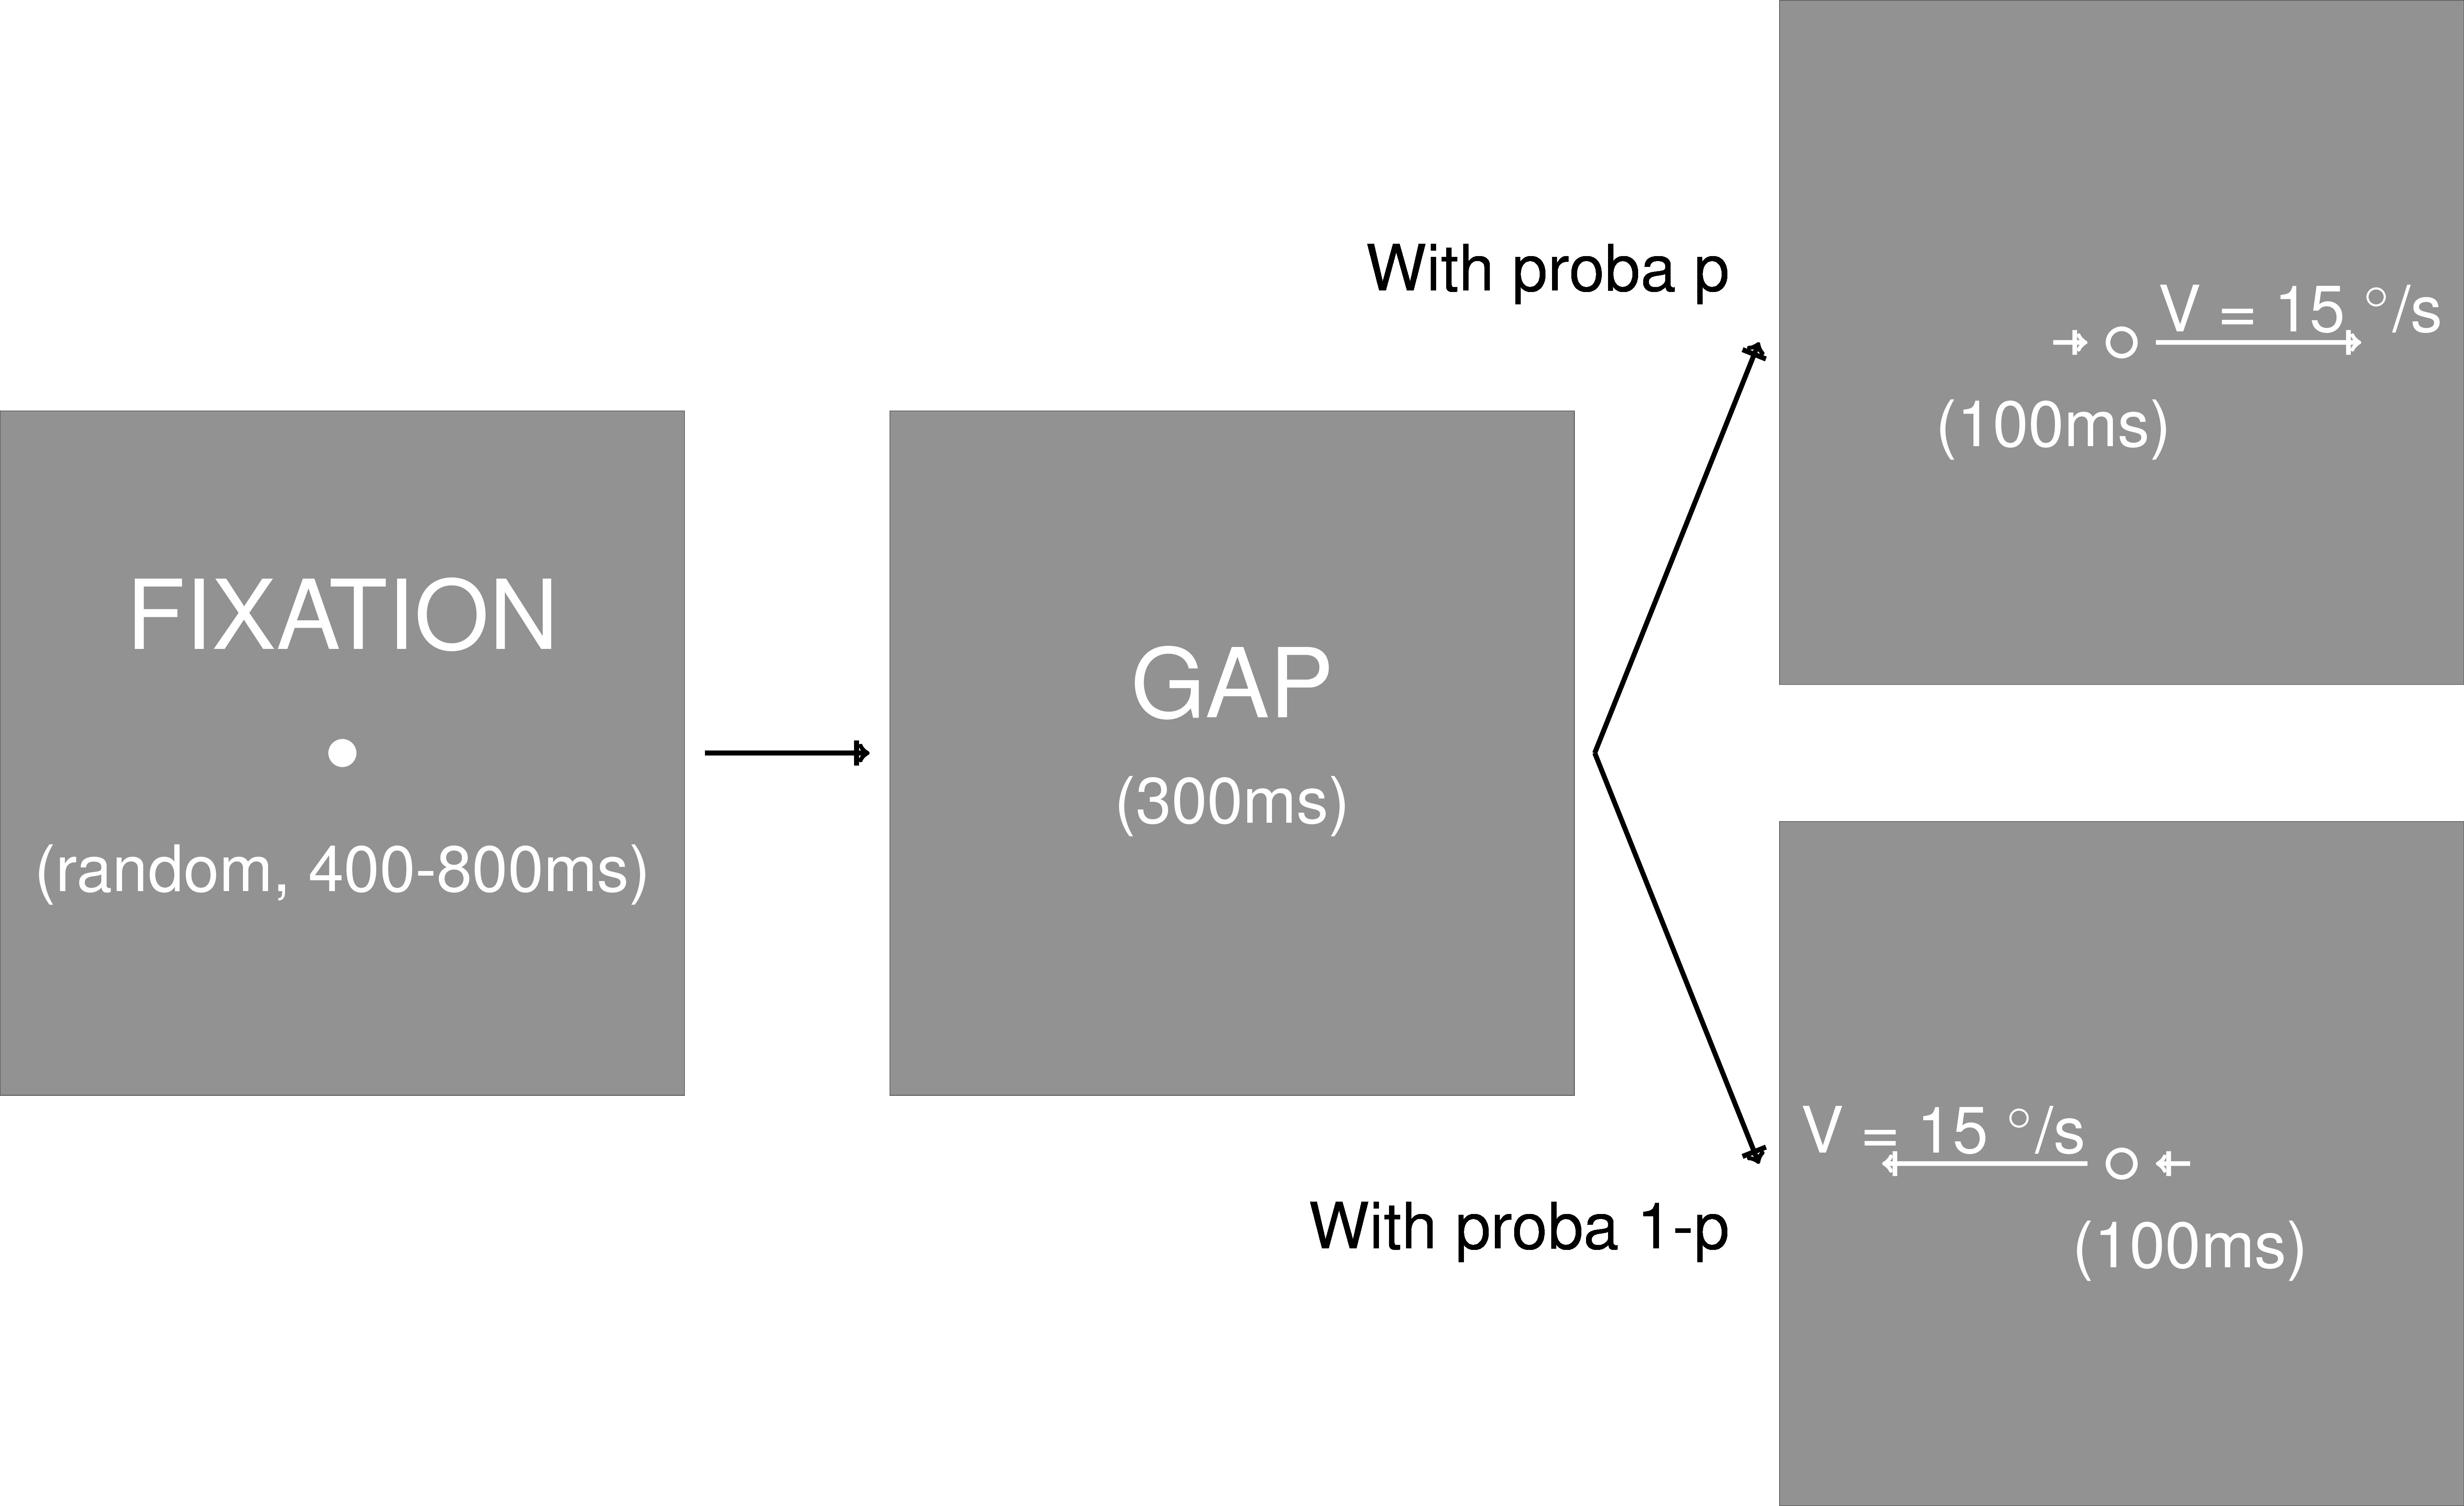
\includegraphics[width=0.333\linewidth]{protocol_recording}};
% cf 3_Results_2.ipynb ??
\node [anchor=north west]  (img2) at (0.333\linewidth,.618\linewidth){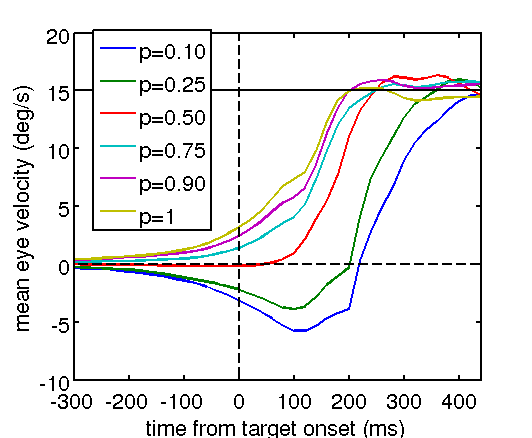
\includegraphics[width=0.333\linewidth]{image_anna_1}};
% cf 0_protocole.ipynb
\node [anchor=north west]  (img2) at (0.666\linewidth,.618\linewidth){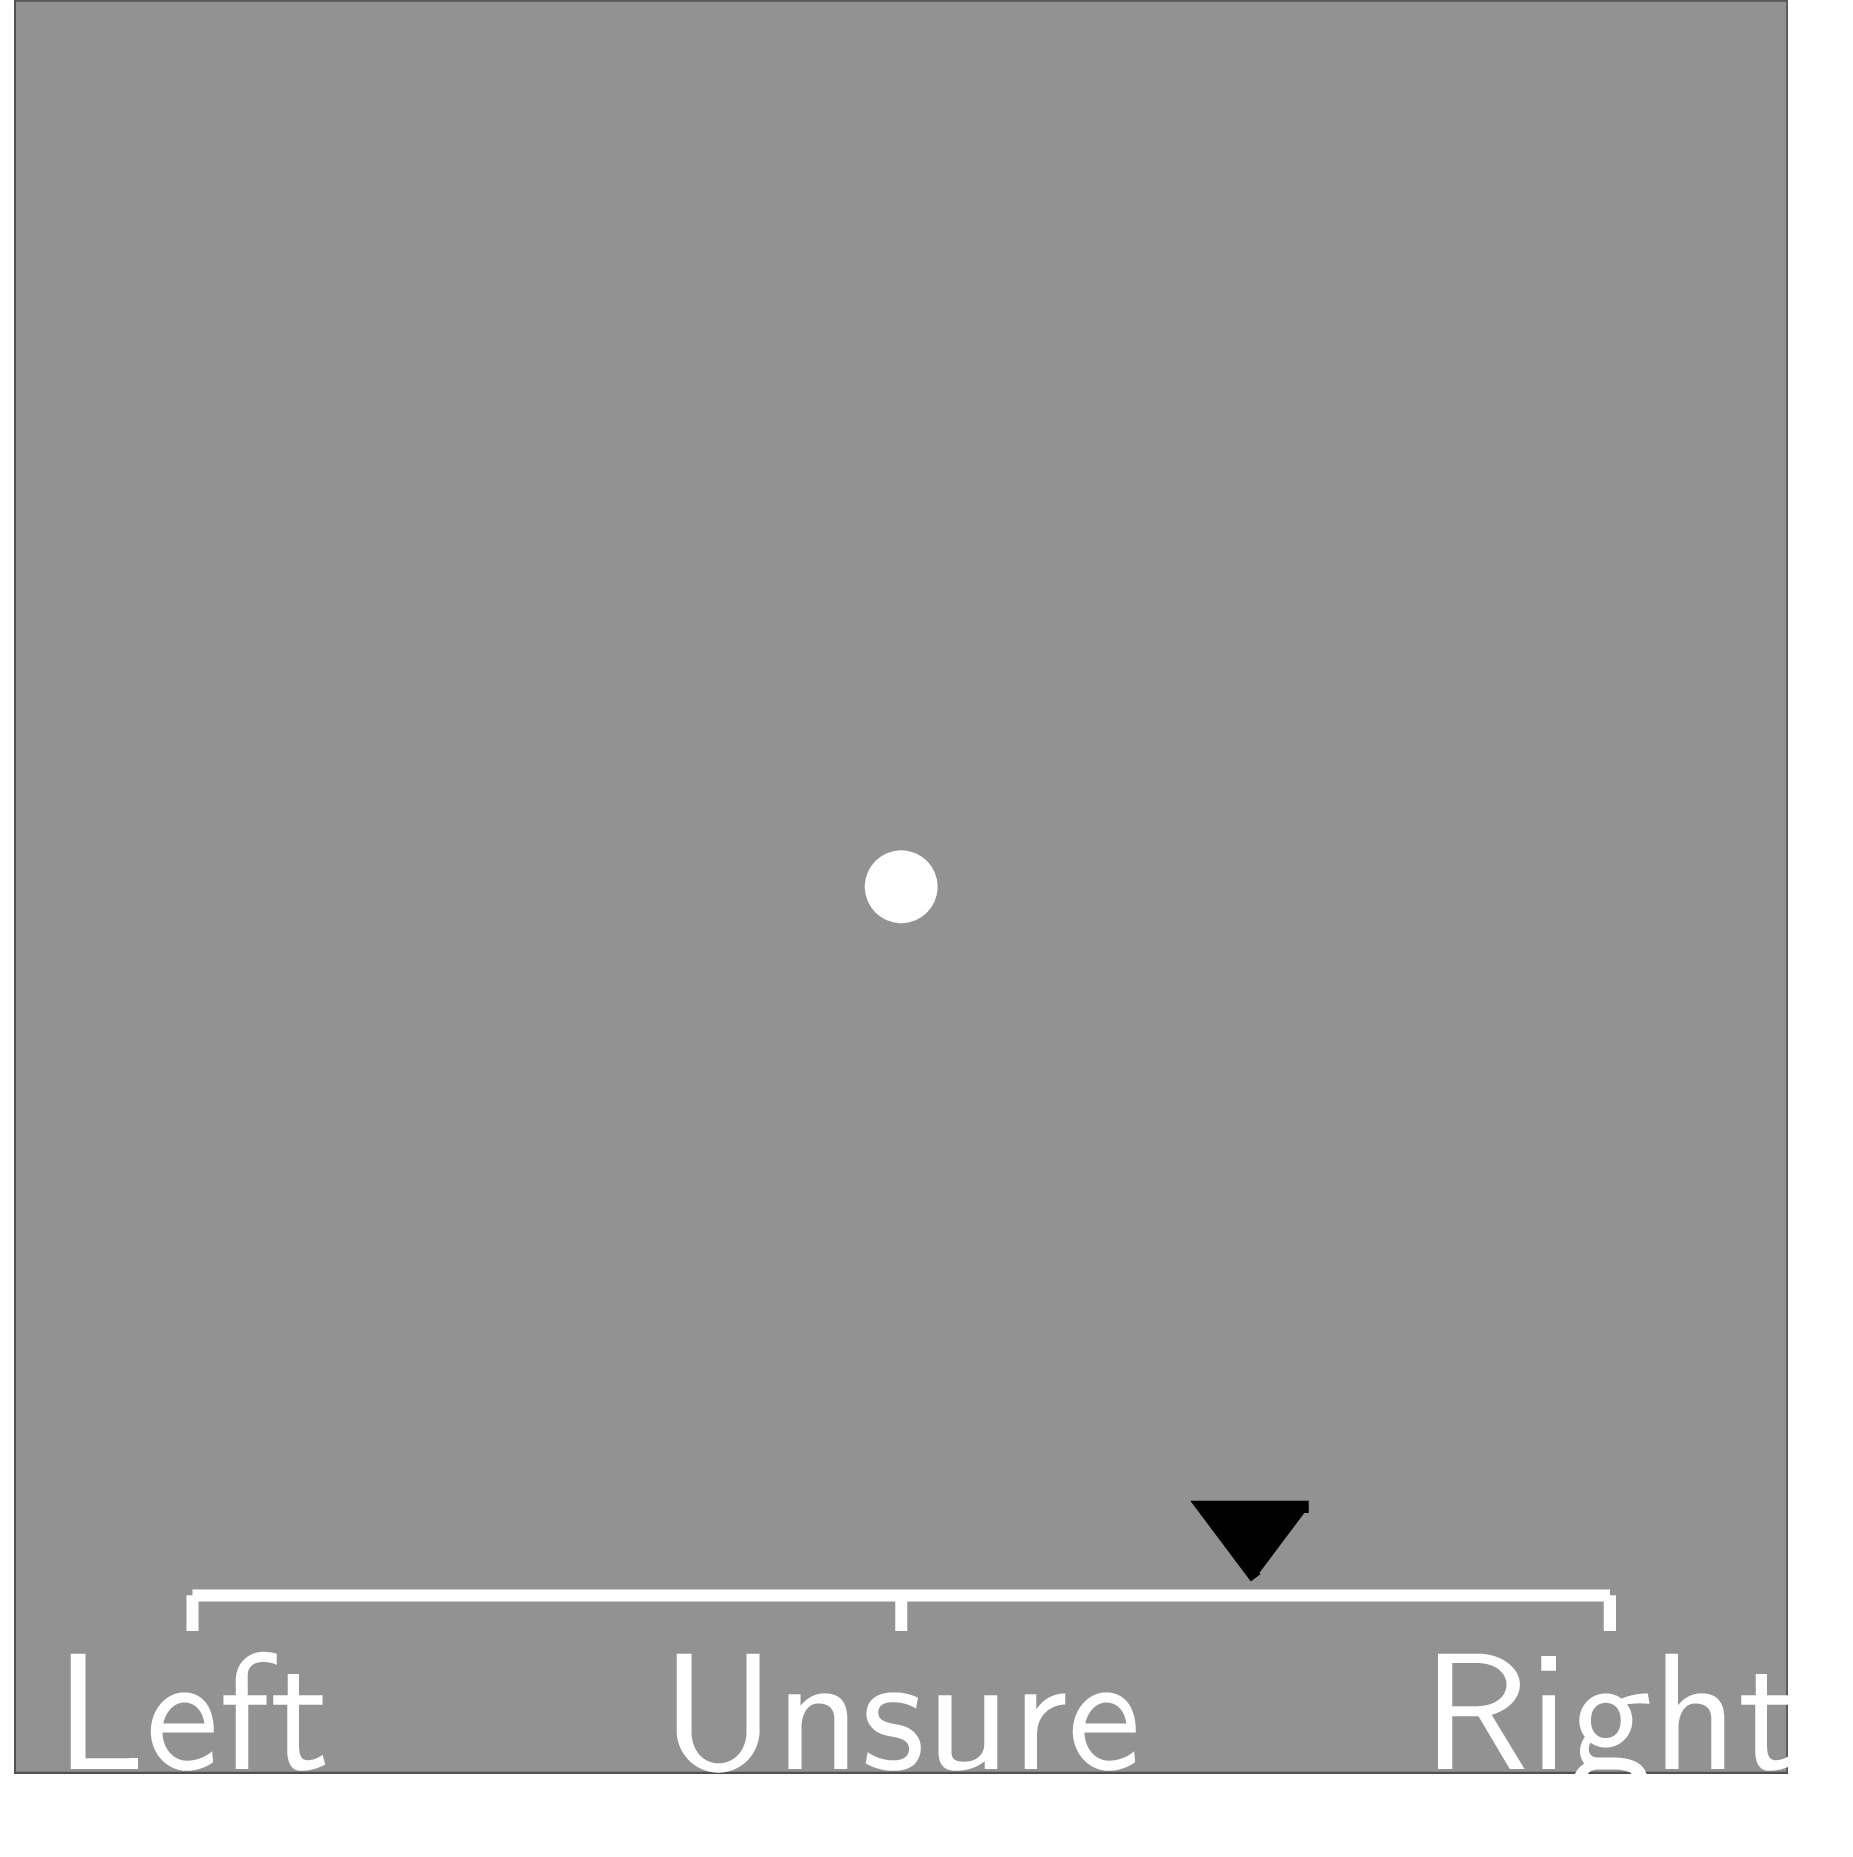
\includegraphics[width=0.25\linewidth]{protocol_bet_simple}};
\draw [anchor=north west] (0.000\linewidth, .618\linewidth) node {$\mathsf{(A)}$};
\draw [anchor=north west] (0.333\linewidth, .618\linewidth) node {$\mathsf{(B)}$};
\draw [anchor=north west] (0.666\linewidth, .618\linewidth) node {$\mathsf{(C)}$};
\end{tikzpicture}
}
\caption{\emph{Anticipatory SPEM (aSPEM): psychophysics and results} %
\textbf{(A)} Human observers were presented $600$ trials
which each consists of sequentially:
a fixation dot (of random duration between $400$ and $600$ \ms),
a blank screen (of fixed duration of  $XXX$ \ms) and
a moving dot (at $15$ deg/s) which the observers were instructed to follow.
The direction of the dot was drawn pseudo-randomly
using a probabilistic bias $p$ which defines the parameter
of the binomial distribution
($0\leq p\leq 1 $ and the direction is unbiased for $p=0.5$,
always left for $p=0$ and always right if $p=1$).
In a first experiment,
we replicated the experiment of~\citep{Montagnini2010} and
tested sequentially for $5$ different values of $p$: $.5$, $.25$, $.75$, $.9$ and $1.$ in fixed blocks of $120$ trials each.
\textbf{(B)}
Velocity traces of eyes movements averaged for each bias condition
over conditions and observers.
These traces are aligned to the onset of the moving dot.
Saccades were removed using a thresholding method~(\seeApp{em}) and
error bars show one standard deviation over all samples.
In the unbiased condition, one can distinguish
a visually driven component (after a latency of $\approx 80 \ms$),
which corresponds to Smooth Pursuit Eye Movements (SPEM).
When introducing a bias in the direction,
one observes that the velocity of the eye progressively ramps
in the direction of the bias and before any visually-guided componentnt:
This phase is the Anticipatory SPEM (aSPEM).
As reported previously~\citep{Montagnini2010, SantosKowler2017},
the slope of this ramp correlates with the strength of the bias.
This is shown in the inset showing the average gain in velocity ($\pm$ SEM)
before any visually driven information (here, at $t=50 \ms$).
\textbf{(C)} In this paper, we extended the experiment in two aspects.
First, we generalized the generation of random sequences
by using random-length blocks
to avoid potential inter-blocks confounds (\seeFig{results_psycho}).
Second, to asses this adaptive mechanism at the conscious level,
we asked each observer to perform the same experiment on a subsequent day,
but with different instructions.
Indeed, we simply asked to rate the level of confidence
for their estimate of the direction of the dot before each trial.
This was performed by moving a mouse cursor on a rating scale
beween "sure left", to "unsure" and finally "sure right".
Eye movements were not recorded.
Due to the random nature of the sequence no observer noticed
that the same pseudo-random sequence was used in the experiment.
 }
\label{fig:intro}
\end{figure}
%-------------------------------------------------------------%
%: adaptation to volatility in EMs : seen as an anticipation in SPEM - principle and function (talk about santos & kowler and others)
% % TODO add saccadic adaptation
Humans are able to accurately track a moving object
with a combination of saccades and
Smooth Pursuit Eye Movements (SPEM)~\citep{ref}.
These movements allow us to align and
stabilize the object on the fovea,
thus enabling high-resolution visual detection.
This process is retarded by different factors such as axonal transduction,
neural processing and the inertia of the oculomotor system~\citep{Krauzlis}.
When predictive information is available about target motion,
anticipatory smooth pursuit eye movements (aSPEM) are
efficiently generated before target appearance,
which reduce the typical sensorimotor delay
between target motion onset and foveation~\citep{PerrinetAdamasFriston2014}.
It is generally assumed that the role of anticipatory eye movements is
to limit the behavioral impairment due
to eye-to-target position and velocity mismatch and
of the variability introduced by neural noise~\citep{WolpertXXX}.

%: how we do it
Repeated presentation of stimulus can lead the oculomotor system
to initiate aSPEM ahead of the stimulus appearance~\citep{Westheimer1954, Kowler1979a, Kowler1979b}.
It has been observed that aSPEM increase in velocity
when the target repeatedly moves in the same direction~\citep{Kowler1984, Kowler1989, Heinen2005}.
Thus,~\citet{Maus2015} have recently shown that
both perceptual adaptation and priming of aSPEM could occur simultaneously.
They found a robust repulsive adaptation effect
with perceptual judgements being biased faster
after seeing stimuli that were slower and~\textit{vice-versa}.
This study clearly shows the integration of past event and
their usefulness in actual eliciting of movements.
Indeed, both priming and adaptation can hypothetically share
a common internal representation of stimulus speed
that has been build upon the mean velocity of last encountered speeds.
Then the comparison of the internal representation of speed
with the current stimulus velocity could explain repulsive aftereffects and
at the same time, be used to elicit aSPEM
of appropriate velocity for next stimulus occurrences.
~\citet{Maus2015} main conclusion was that
perceptual adaptation and oculomotor priming
both have a weight in building an~\textit{a priori} knowledge
that will be used to generate aSPEM.
Still, they integrated past history over different times scales
with the priming effects being maximized
for short stimulus histories (around 2 trials) and
adaptation for longer stimulus history, around 15 trials.
Such history length can still be considered
short history namely in the case of several hundreds blocks
of trials like we did in our first study.

%: in summary we get a linear relationship
Throughout the first experimental condition,
we investigated the integration of environmental statistical regularities
in a smooth tracking task with
a family of direction-biases for the target motion.
What we found was a global and robust effect of direction-bias
on anticipatory smooth pursuit.
These results are coherent with previous oculomotor findings
by our and also other groups~\citep{Montagnini2010, SantosKowler2017}.
Typically, aSPEM is observed after a temporal cue and
ahead of target motion onset (Kowler and Steinman, 1979a,b, 1984).
Some now classical experiments have demonstrated the existence
of prediction-based smooth pursuit during
the transient disappearance of a moving ~\citep{Badler2006,BeckerFuchs, 1985}.
Overall, it is now clear that smooth pursuit behavior
can be modulated even in the absence of online sensory stimulation.
aSPEM were here the core of our research because
we wanted to study the trial-by-trial evolution
of expectancy-based oculomotor behavior,
as well as how sensorimotor expectancy interacts
with reward contingencies in shaping oculomotor behavior
without direct sensory feedback.
In a previous study,~\citep{SoutoMontagniniMasson2008, Montagnini2010},
we have analyzed how forthcoming motion properties,
such as target speed or direction, can be
predicted and anticipated with coherent orienting eye movements.
We found a graded effect of both the speed and the direction-bias,
with mean anticipatory eye velocity
linearly related to the probability of motion's speed or direction.
Here, we replicated part of those results
using a limited number of direction probability bias and
strengthened them by generalizing them on seventeen participants.
These results imply that the probability bias over a target's direction is
one additional factor beyond other physical and cognitive cues~\citep{Kowler2014, SantosKowler2017},
that modulate the common predictive framework
driving anticipatory behavior to optimize a rapid and
precise foveation of the target on its most expected future path.

% --------------------------------------------------------------------------------------
\subsection{Contributions}%Outline}
% --------------------------------------------------------------------------------------
%: limits of the previous method
The goal of this study is to generalize the adaptive process
obesrved in aSPEM to more ecological settings but
also to broaden its scope by showing that such unconscious process
also occurs at the conscious level.
Indeed, by manipulating the probability for target motion direction,
we were able to bias the direction and mean velocity of aSPEM,
as measured during a fixed duration gap
before target ramp-motion onset~(\seeFig{intro}-A \& B).
This suggests that probabilistic information may be used
to inform the internal representation of motion prediction
for the initiation of anticipatory movements~\citep{Montagnini2010}.
First, one possible confound in the previous study was
to use a sequence of blocks of conditions on $p$ with fixed lengths.
Indeed, observers could potentially pick up
the information on this fixed length
In particular, we observed that following the switch from
one condition to the next,
the strength of aSPEM changed gradually,
consistently with other adaptation paradigms~\citep{SoutoXXSacadicAdaptation},
but for which the adaptation mechanism was only fitted.
As a consequence, such estimate may become particularly
challenging in a dynamic context,
where the probabilistic contingencies vary in time in an unpredictable way.
In addition, whether and how the information processing underlying
the buildup of aSPEM and its dynamics is linked to
an explicit estimate of probabilities is unknown.
To alleviate this problem, we developed a new paradigm
in order to address this question
by explicitly modeling a dynamic process with a given volatility.

%\subsection{Generative model: the binomial switching model}
%-------------------------------------------------------------%
%:  FIGURE 2 fig:results_raw
\begin{figure}%[b!]
\centering{
\begin{tikzpicture}%[thick,scale=1, every node/.style={scale=1} ]
	% cf 1_generative-model.ipynb
	\node [anchor=north west]  (img1) at (0.000\linewidth,.618\linewidth){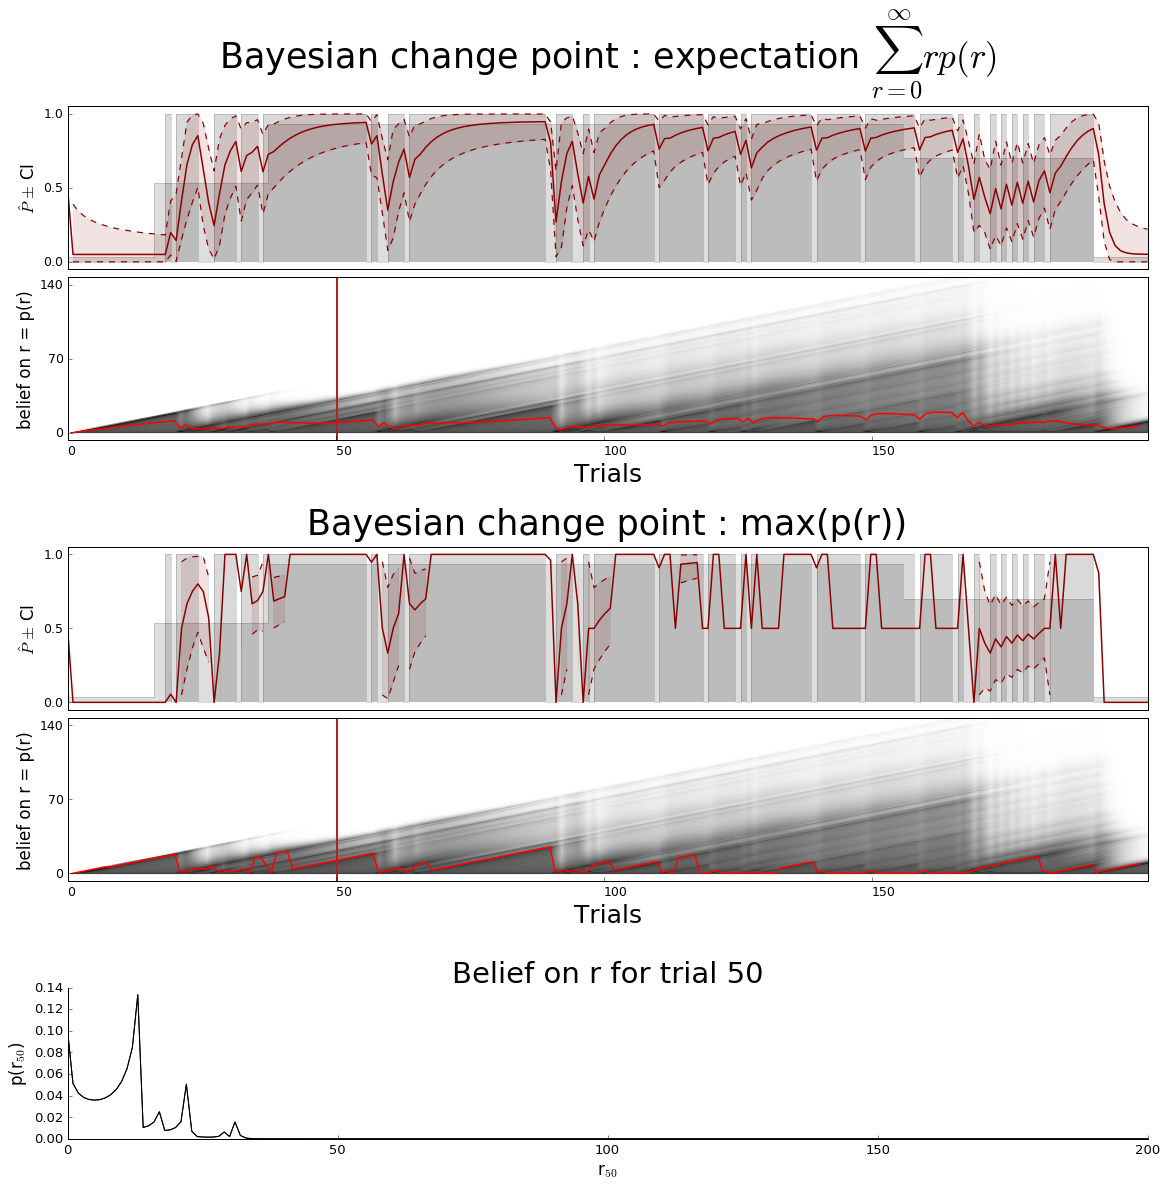
\includegraphics[width=0.2\linewidth]{bayesianchangepoint}};
	% cf 3_Results_2.ipynb ??
	\node [anchor=north west]  (img2) at (0.200\linewidth,.618\linewidth){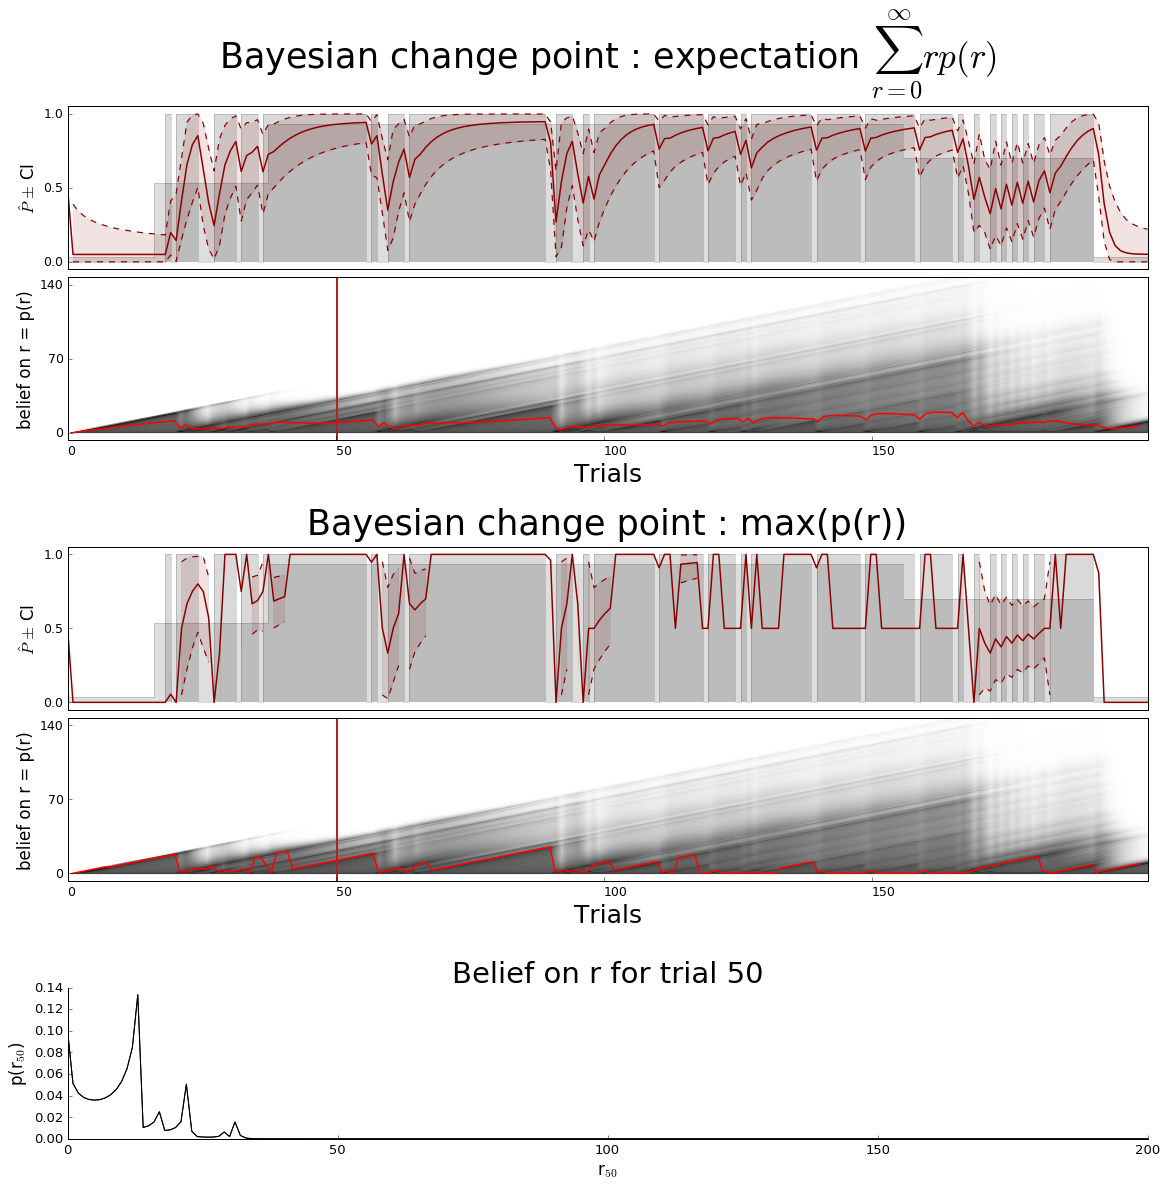
\includegraphics[width=0.8\linewidth]{bayesianchangepoint}};
	% cf 0_protocole.ipynb
	\draw [anchor=north west] (0.000\linewidth, .618\linewidth) node {$\mathsf{(A)}$};
	\draw [anchor=north west] (0.200\linewidth, .618\linewidth) node {$\mathsf{(B)}$};
\end{tikzpicture}
}	% cf 2_Methodes.ipynb ??
% ou cf 3_Results_2.ipynb
\caption{%
\emph{The binomial switching model and raw Psychophysical results}%
~\textbf{A}
This diagram represents the stochastic model chosen
to generate the sequence of directions.
It is represented as a graphical model representing
the three levels of the stochastic model. %
~\textbf{B}
%
% * I show here the overlay of this variable on the plot of
%  probability biases
%
% * these accelarations values were here scaled according
% to their extremal values.
%
% * there seems to be a trend with the polarity of the acceleration
% being negative for p values below .5 and positive for values above .5
%
% To observe the fit in an appropriate range between 0 and 1,
% the data for participant 18 was normalized and
% re-centered with the following transformation method:
% $\widetilde{aSPEM} = \frac{aSPEM_t-Min(aSPEM)}{Max_(aSPEM)-Min(aSPEM)}$.
%
Raw results for one characteristic observer.
In this plot we superpose the sequence of event
(red or black dots for respectively left or right directions),
the (hidden) evolution of the value of $p$ (horizontal black segments)
and the underlying times for switches (vertical black lines).
Note that we introduced pauses every  $50$ trials to prevent from fatigue.
% Each block is divided in 4 sub-blocks of $50$ trials as denoted by vertical black bars
Using a pseudo-random number generator with the same seed,
we could present the exact same sequence to all subjects. %
We have superposed the trace of
1/ the aSPEM strength as measured by the horizontal displacement
at the onset of the visually-driven SPEM (red line),
2/ the response to the bet experiment (red line) and
3/ the result of the BCP model (blue line)
along with the confidence interval for this estimate (blue shaded area).
}
\label{fig:results_raw}
\end{figure}
%-------------------------------------------------------------%
%: design of the binomial switching generative model
Indeed, to assess the dynamics of the adaptive processes
which compensate for the variability of sensory,
one may introduce a parametric mechanism controlling for its volatility.
By definition, volatility measures the temporal variability
of the sufficient parameters of a random variable.
In the HGF model~\citep{Matthys2011} for instance,
volatility is modeled as the non-linear transformation
of a random walk (modeled itself by a Brownian motion).
This models allows to generate a sequence of binary choices
where the variability fluctuates along a given trajectory.
Such a forward probabilistic model is invertible
using some simplifying assumptions and allows
to extract an inference of the agent's belief about volatility~\citep{Voessel??}.
Herein, we will use a simpler model where
The probability of this process varied in a piecewise-constant
(that is, a step function varying between~$0$ and~$1$),
similarly to~\citet{Meyniel13}.
For each trial, a target makes either to the left or to the right,
and we denote this variable as $x_0^t$ at trial $t$.
This direction being drawn from a Bernoulli process $\Bb$
with a parameter that we define as $p=x_1^t$.
The novelty is that this variable is chosen
at random from a prior distribution $\Pp$ at the moment of a switch.
The occurrence of these switches is itself drawn from a Bernoulli process
of probability $1/\lambda$.
Mathematically, this is easily described
by a graphical model~(\seeFig{results_psycho}-A) and
the following definition:
\eql{\choice{
x_0^t \eqdef o_t \propto \Bb(p^t) \\
x_1^t \eqdef p_t = p_{t-1} \quad \text{if} \quad s_t=0 \quad \text{and else} \quad p_t \propto \Jj \\
x_2^t \eqdef s_t \propto \Bb(1/\lambda)
}\label{eq:sgm}}.
Note that the prior distribution $\Pp$ can be for instance
the uniform distributions on $ [ O, 1 ] $ or
Jeffrey's prior~\seeApp{bcp}(TODO: put in appendix).
There is always a switch at $t=0$ and for each pause.
In conclusion, the experimental setup of the first session
is similar to that presented in~\seeFig{intro}-A, except for
this new generative model for the pseudo-random sequence of binary events
~\seeFig{results_psycho}-B.

%: outline
This paper is organized in five parts.
After this introduction, the next section will present
an inversion of the forward probabilistic model defined in~\seeEq{sgm}.
There is yet no such algorithm to our knowledge and
we will here provide with a solution
by extending previous results from~\citet{AdamsMackay2007}
to the case of binomial data.
We will also provide with a computational implementation
and a quantitative evaluation of this algorithm.
Then, we will present psychophysics on eye movements
to validate the generalization of previous results
In a first session, participants observe a target moving horizontally
with constant speed from the center
either to the right or left across trials~(\seeFig{intro}-A).
The probability of either motion direction changes randomly in time.
In a second session, participants are asked to estimate
"how much they are confident that
the target will move to the right or left in the next trial" and
to adjust the cursor's position on the screen accordingly~(\seeFig{intro}-C).
In the fourth part, we will analyze the inference of the volatility
for each individual participant.
This will allow the analysis of inter-individual changes for each session
and in particular in one could predict one's prior volatility,
that is, a measure of the dynamic compromise between exploration and exploitation
across the two different sessions testing predictive adaptive processes
at the unconscious and conscious levels.
Finally, we will summarize and conclude this study and
offer some perspectives for future work.
%: %%%%%%%%%%%%%%%%%%%%%%%%%%%%%%%%%%%%%%%%%%%%%%%%%%%%%%%%%%%%%%%
\section{Results: Bayesian change point model}

% These python scripts are available at \url{https://github.com/laurentperrinet/bayesianchangepoint}.
%TODO include changing point theory and bibliography
% TODO : check http://www.princeton.edu/~rcw2/papers/WilsonEtAl_PLOSCompBiol2013.pdf and bernouilli case + evaluation



See Matthys

Necessity of using a generative model


\subsection{Forgetful-agent model (Leaky integrator)}
% it's a particular case of the solution to the generative model assumaing a fixed -block length
%
% Following the~\citet{Maus2015} analysis, we performed a first study~page~\pageref{chap:4} in which we wanted to test a more realistic model of how trial-history shapes motion expectation in a direction-biased experiment.  According to~\citet{Anderson2006}, the temporal evolution for the expectation of a given event can be modeled making a simple assumption: the update of the estimated probability for an event is based on the discount of the previous estimated probability by a factor$~\lambda$, relative to new information. The value of$~\lambda$ presumably represents a compromise between responding rapidly to genuine changes in the environment and not prematurely discarding information still of value for slowly changing contexts. We extended~\citet{Anderson2006}'s approach to our analysis of anticipatory smooth pursuit across different contexts corresponding to the experimental blocks with different global probability-bias. We designed a forgetful agent estimating the target motion direction-bias according to the following iterative equation, where the estimated probability of a target moving rightwards is obtained from (1) the previous bias inference, (2) the imposed target directions and (3) a memory decay in the weighting of information. This model can be explained with the following equation:
%
%
%\[\hat{p}_{0} = 0.5\]
%\[\hat{p}_{i+1} = (1 - 1/\tau)*\hat{p}_{i} + 1/\tau * \textit{D}_{i}\]
%
%where
%\begin{enumerate}[label={}]
%\item $\hat{p}_{i}$ = estimation of rightward trials probability at trial~\textit{i}
%\item $\tau$ = characteristic memory decay time (in trials for the inference of $p$)
%\item $\textit{D}_{i}$ = Imposed directions. Sequence of 0 (leftward) and 1 (rightward) trials
%\end{enumerate}
%
% We simulated the sequence of p-estimates of the forgetful agent for each direction-bias block and for different values of~$\tau$. Fig~\ref{fig:p_est.pdf} below illustrates, for the $p=90\%$ direction bias block, the intuitive notion that with a small value for~$\tau$~(or equivalently a volatile memory) the agent's estimate is more sensitive to changes in the target direction trial sequence. On the other hand,  with larger~$\tau$~like 40 or 50, the estimation of p tends to fluctuate only very mildly around the global direction-bias over the experimental block.
%
%\begin{figure}[H]
%\centering
%\begin{subfigure}{1\textwidth}
%\includegraphics[width=1\textwidth]{p_est.pdf}
%\phantomcaption{\label{fig:p_est.pdf}}
%\end{subfigure}
%\caption[A forgetful-agent]{The forgetful agent's $p$-estimations with different values of~$\tau$ for the $p=90\%$ direction-bias block\label{fig:p_est.pdf}}
%\end{figure}
%
% Then, we performed a linear regression analysis of the relation between the experimentally measured anticipatory eye velocity and the simulated estimate of p for each direction-bias block. To do so, we again pooled together the eye movement velocity from all participants in each experimental condition and along the direction-bias estimated by the model at the time of their triggering. We then estimated the correlation coefficient $R$ as a function of~$\tau$. We found that $R$ is maximised for~$\tau = 5$ in $p = 50\%$ blocks ($R=.18$, $p<.05$) and $p = 75\%$ blocks ($R=.27$, $p<.05$) , and for~$\tau = 10$ for $p = 90\%$ blocks ($R=.32$, $p<.05$) (see Fig~\ref{fig:R_BL.pdf}). The correlation coefficient decreases for higher values of~$\tau$, coherent with the previous study from~\citet{Maus2015} from which we inspired this analysis. Still, the overall $R$ values are slightly higher compared to the raw linear regression with the unweighted fixed-size memory, indicating a better performance of this "forgetful" agent model.
%
%\begin{figure}[H]
%\centering
%\begin{subfigure}{1\textwidth}
%\includegraphics[width=1\textwidth]{R_BL.pdf}
%\phantomcaption{\label{fig:R_BL.pdf}}
%\end{subfigure}
%\caption[Pearson's R between experimental data and forgetful agent]{Linear regression coefficient R as a function of~$\tau$~$(1/\lambda)$ . This quantity is a rough estimate of the matching between the simulated p-estimates by the forgetful agent and experimental anticipatory eye velocity.\label{fig:R_BL.pdf}}
%\end{figure}
%
% We then looked at the linear relation of experimental data with the probability bias estimated by the model throughout all direction blocks for all our participants with~$\tau = 10$ and as we can see on Fig~\ref{fig:P_VEM_vs_pestBL.png}, we found a graded relation between Pearson's $R$ with  $R = .17$ ($p<.05$) in $p = 50\%$ blocks, $R=.27$ ($p<.05$) in $p = 75\%$ and $R=.30$ ($p<.05$) in $p = 90\%$ blocks. This shows that anticipatory smooth eye velocities are somehow related to the estimation of $p$ given by a forgetful agent. The overall computation of this analysis to all our condition showed, coherently with~\citep{Maus2015} (see study~\ref{chap:4},~page~\pageref{chap:4}), a tendency of having higher R's for short-memory, independently of the experimental condition (see Fig~\ref{fig:R_summary_2.pdf}). Though, it is important to note a better fitting quality for this using the forgetful-agent model as in~\citet{Anderson2006}.
%
%\begin{figure}[H]
%\centering
%\begin{subfigure}{1\textwidth}
%\includegraphics[width=1\textwidth]{P_VEM_vs_pestBL.png}
%\phantomcaption{\label{fig:P_VEM_vs_pestBL.png}}
%\end{subfigure}
%\caption[Anticipatory smooth velocity classified by the estimated probability bias]{Linear regression of anticipatory velocities in function of a~$\tau$~$(1/\lambda)$ = 10 estimation. \label{fig:P_VEM_vs_pestBL.png}}
%\end{figure}
%
%\begin{figure}[H]
%\centering
%\begin{subfigure}{1\textwidth}
%\includegraphics[width=1\textwidth]{R_summary_2.pdf}
%\phantomcaption{\label{fig:R_summary_2.pdf}}
%\end{subfigure}
%\caption[Relation between P-estimation and experimental conditions]{Linear regression of anticipatory velocities in function of a~$\tau$~$(1/\lambda)$ = 10 estimation for each conditions. \label{fig:R_summary_2.pdf}}
%\end{figure}
%
% To conclude on this section, the "forgetful agent" computed an exponentially-weighted moving average and estimated the probability of a stimulus going to the right given the previous instances of rightward stimulus and a progressive discount of past information. When we looked at the relation between aSPEM velocities and the direction-bias estimated by our model, we found higher Pearson's R for short-term memory ($\approx$ 5 to 10 trial history lengths) rather than long-term memory. However, a first critic could be that our proposed model may be too rigid and does not sufficiently imply the concepts of volatility~\citep{Behrens2007} or Bayesian uncertainty~\citep{Vilares2011}. It seems plausible that the memory (history length) the brain uses for inference is varying and that this variation could be related to the volatility inferred from information in the past. For instance, our model could not be applied to $p = 100\%$ rightward direction blocks because of a pretty quick saturation toward an estimation of probability equal to 1 even though experimental aSPEM datas shows a weak but existing proportion of aSPEM to the left direction. To address this hypothesis, our next model work will be inspired by a Bayesian Change-point detection model~\citep{Adams2007}, which mimics an ideal agent inferring both the likelihood of a specific event's occurrence with the volatility of the environment (e.g the duration since a change in bias).
%



\subsection{Bayesian change point model}

We have designed an agent adapted the Bayesian Online Change-point Detection model~\citep{AdamsMackay2007}. This model uses a latent variable r which represents the length of the current interval during which motion-direction probability ($\hat{P}$) has not changed. The agent infers at each trial the likelihood  of r and then deduces the optimal $\hat{P}$ (we used the expected value and the max as readouts) and the uncertainty associated to it. We simulated the model across our experimental sequences, as illustrated by the example for the third block.


%* an implementation of
%%[Adams &amp; MacKay 2007 "Bayesian Online Changepoint Detection"](http://arxiv.org/abs/0710.3742)
%in Python.
%
%````
%@TECHREPORT{ adams-mackay-2007,
%AUTHOR = "Ryan Prescott Adams and David J.C. MacKay",
%TITLE  = "Bayesian Online Changepoint Detection",
%INSTITUTION = "University of Cambridge",
%ADDRESS = "Cambridge, UK",
%YEAR = "2007",
%NOTE = "arXiv:0710.3742v1 [stat.ML]",
%URL = "http://arxiv.org/abs/0710.3742"
%}
%````
%
%* adapted from https://github.com/JackKelly/bayesianchangepoint by Jack Kelly (2013) for a binomial input.
%
%* This code is based on the  [MATLAB implementation](http://www.inference.phy.cam.ac.uk/rpa23/changepoint.php) provided by Ryan Adam. Was available at http://hips.seas.harvard.edu/content/bayesian-online-changepoint-detection
%
% * full code @ https://github.com/laurentperrinet/bayesianchangepoint


%-------------------------------------------------------------%
%:  FIGURE 3 fig:bayesianchangepoint \seeFig{bayesianchangepoint}
%: TODO présente le principe de l'algorithme, le résultat sur une séquence et une aanlyse quantitative qui permettra de l'utiliser pour les expériences psycho
\begin{figure}%[b!]
\begin{center}
% cf 3_Results_2.ipynb
    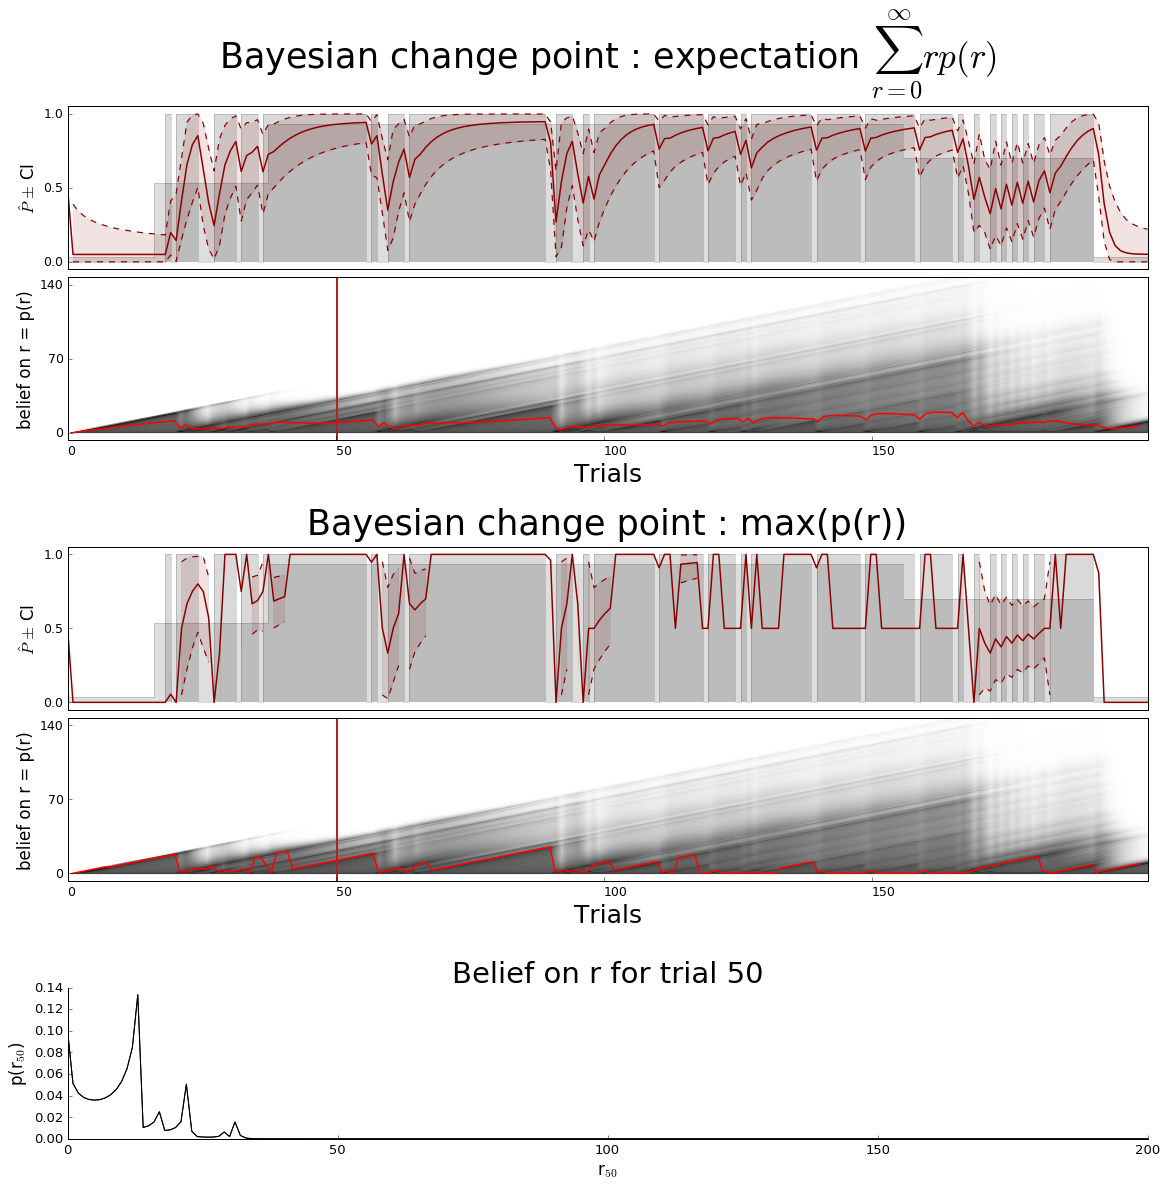
\includegraphics[width=1\linewidth]{bayesianchangepoint}
\end{center}
\caption{\emph{Bayesian change point model}~\textbf{A} shows hypothetic datas that works as a binomial choice, either 0 (leftward) or 1 (rightward). In particular, the probability switched at trials 6 and 10.~\textbf{B} shows the graph (treillis) on which the message indicates that mass probability is being passed. Black lines denotes "upwards", that is, for which there is a progression of the run length at the next step. The red line stands for the possibility that a switch happened, and then falls back to zero. The black curve stands for the run length of simulated datas in~\textbf{A} in function of time (r$_t$). We can see that the run length drops back to zero when change occurs at trials 6 and 10.
%\textbf{(C)}
%* in this graph information will be represented at different nodes. each node represent a belief which takes the form of a probability distribution over the set of parameters that we wish to describe.
%* it can be the mean and variance of a Gaussian, but in general it will be 2 parameters. in our case, we wish to estimate p (between zero and one) - it is characterized by the beta distribution (mathematically it is the conjugate of the bernouilli distribution)
%* (mathematically, we will use th family of exponenetial distributions:, gaussians, binomials) among which the beta distribution belongs
%First, we initialize the first node to prior values
%* at trial zero, there is no information, so we intiialize to the prior values
% use p log p + (1-p) log (1-p ) as in logistic regression?
% TODO show fit with different hazard rates
}
\label{fig:bayesianchangepoint}
\end{figure}
%-------------------------------------------------------------%


Fig~\ref{fig:BCP_figA}~\textbf{A} shows one instance of a sequence of simulated datas of leftward and rightward trials with a probability $p$ of being rightward with possible variations through times. It also shows the predicted probability $\hat{p}$ by using the BCP algorithm. Fig~\ref{fig:BCP_figB} illustrates the belief r on the predicted probability $\hat{p}$ at a given trial. On Fig~\ref{fig:BCP_figC} and Fig~\ref{fig:BCP_figD}, we can see the belief on the run length estimation.

Note, the fixed-length is imply implemented by a (broken) line with fixed run-length $r_t=\tau$) - this allows for a simple comparison

\subsection{Bayesian change point algorithm}

%cf p33 de 2018-02-12 journal club bayesian changepoint chloe.pdf

% Fig~\ref{fig:BCP_figA}~\textbf{A} shows one instance of a sequence of simulated datas of leftward and rightward trials with a probability $p$ of being rightward with possible variations through times. It also shows the predicted probability $\hat{p}$ by using the BCP algorithm. Fig~\ref{fig:BCP_figB} illustrates the belief r on the predicted probability $\hat{p}$ at a given trial. On Fig~\ref{fig:BCP_figC} and Fig~\ref{fig:BCP_figD}, we can see the belief on the run length estimation.
%
%\begin{figure}[H]
%\centering
%\begin{subfigure}{1\textwidth}
%\includegraphics[width=1\textwidth]{BCP_fig.pdf}
%\phantomcaption{\label{fig:BCP_figA}}
%\end{subfigure}
%\begin{subfigure}{0\textwidth}
%\includegraphics[width=1\textwidth]{BCP_fig.pdf}
%\phantomcaption{\label{fig:BCP_figB}}
%\end{subfigure}
%\begin{subfigure}{0\textwidth}
%\includegraphics[width=1\textwidth]{BCP_fig.pdf}
%\phantomcaption{\label{fig:BCP_figC}}
%\end{subfigure}
%\begin{subfigure}{0\textwidth}
%\includegraphics[width=1\textwidth]{BCP_fig.pdf}
%\phantomcaption{\label{fig:BCP_figD}}
%\end{subfigure}
%\caption[Bayesian Change Point model computation]{~\textbf{A} is a sequence of points representing leftward (0) of rightward trials (1) with a given probability $p$ of being rightward and that changes at some trials (clear red). The predicted probability $\hat{p}$ ($\tau=N_{trial}/4$ tells the BCP that the probability is more susceptible to change every $N_{trial}/4$), continue and dotted dark red lines shows the $p$$-$estimation.~\textbf{B} shows the probability of the run length, the probability of the having same probability consecutive trials. The red line represents the $\hat{r}$, that represents the sum of he products of each r (number of consecutive trials having the same probability)  $\sum_{r=0}^\infty r \cdot P(r)$.~\textbf{C} represent the probability of each r for trials 50 and 250 along their $\hat{r}$ and their $\hat{p}$. For instance, for trial 50, we can observe that $\hat{r}$ is close from the real number of trials during the probability has not change (real $p$ stayed for 50 trials). $\hat{p}$ is also pretty close from the real $p$ ($p=1$).~\textbf{D} shows that at trial 250 $\hat{r}$ is more far than the real r that is also equal to 50 trials. But here, $\hat{p}$ is closer from $p$ that is equal to 0.75. \label{fig:BCP_fig.pdf}}
%\end{figure}
%
% We adapted this model to the data our first study,~page~\pageref{chap:4}, by taking the alternating output of leftward/rightward trials as the sequence of observations that will be under the analysis of the model. This model uses a latent variable r which represents the length of the current interval during which motion$-$direction probability~($\hat{p}$)~has not changed. The agent infers at each trial the likelihood of r and then deduces the optimal~$\hat{p}$~(we used the expected value and the max as readouts) and the uncertainty associated to it. Finally, the whole algorithm simplifies to the following iterations:

Following the principle of Active Inference,
To summarize, the algorithm % uncover progressively

\begin{enumerate}
	\item     Initialize

	\begin{itemize}
		\item    $P(r_0)= S(r)$ or $P(r_0=0)=1$ and
		\item    $\nu^{(0)}1 = \nu_{prior}$ and $\chi^{(0)}1 = \chi_{prior}$
	\end{itemize}

	\item    Observe New Datum $x_t$
    \item    Evaluate Predictive Probability $\pi_{1:t} = P(x |\nu^{(r)}_t,\chi^{(r)}_t)$
    \item    Calculate Growth Probabilities $P(r_t=r_{t-1}+1, x_{1:t}) = P(r_{t-1}, x_{1:t-1}) \pi^{(r)}_t (1-H(r^{(r)}_{t-1}))$
    \item    Calculate Changepoint Probabilities $P(r_t=0, x_{1:t})= \sum_{r_{t-1}} P(r_{t-1}, x_{1:t-1}) \pi^{(r)}_t \cdot H(r^{(r)}_{t-1})$
    \item    Calculate Evidence $P(x_{1:t}) = \sum_{r_{t-1}} P (r_t, x_{1:t})$
    \item    Determine Run Length Distribution $P (r_t | x_{1:t}) = P (r_t, x_{1:t})/P (x_{1:t}) $
    \item    Update Sufficient Statistics :
	\begin{itemize}
		\item    $\nu^{(0)}_{t+1} = \nu_{prior}$, $\chi^{(0)}_{t+1} = \chi_{prior}$
		\item    $\nu^{(r+1)}_{t+1} = \nu^{(r)}_{t} +1$, $\chi^{(r+1)}_{t+1} = \chi^{(r)}_{t} + u(x_t)$
	\end{itemize}

    \item    Perform Prediction $P (x_{t+1} | x_{1:t}) = P (x_{t+1}|x_{1:t} , r_t) P (r_t|x_{1:t})$
    \item    go to (2)
\end{enumerate}

% use that distance to compute optimal hazard rates
where $\KL{\hat p}{p}$ is the Kullback-Leibler divergence between samples $\hat p$ and model $p$ under a Bernouilli distribution
\begin{equation}
\KL{\hat p}{p} = \hat{p} \log\pa{\frac{\hat p}{p}} + (1-\hat p) \log\pa{\frac{1-\hat p}{1-p}}.
\end{equation}


Contrary to the forgetful-agent model where~$\tau$ was a fixed parameter, the BCP use a changing~$\tau$ parameter. In the latter the~$\tau$ parameter informs the BCP model that the probability is suspected to change every~$\tau$ trials. As we can see on~\ref{fig:search_tau.png}, participants do not have the same pattern of responses (examples of participants 16 and 18 below). Still we were able to extract the parameter~$\tau$ that maximizes the fit between the probability computed by the BCP model ($\hat{p}$) and the experimental datas.

%\begin{figure}[H]
%\centering
%\begin{subfigure}{1\textwidth}
%\includegraphics[width=1\textwidth]{search_tau.png}
%\phantomcaption{\label{fig:search_tau.png}}
%\end{subfigure}
%\caption[Correlation maximization in function of  $\hat{p}$ in the BCP model]{This figure shows the evolution of the correlation between $\hat{p}$ and the experimental datas of participants 18 and 16 in function of~$\tau$ (i.e the point where $p$ is suspected to change) for each experimental condition and probability block (color-coded, see legend). Points represent the~$\tau$ that maximizes the correlation between datas and $\hat{p}$ in our different modalities
%\label{fig:search_tau.png}}
%\end{figure}

\hfill \break
 Then we looked at the fit between the probability predicted by the BCP $\hat{p}$ (for the sequences of events (rightward and leftward trials) that we used for our different experimental blocks) and the experimental datas obtained by participants. As we can see on fig~\ref{fig:data_fit_S18.pdf} we have a nice fit between the normalized aSPEM behavioral datas of participant 18 and the probability~$\hat{p}$ computed by the BCP.



%\subsection{Computing the likelihood}
The main difference between our algorithm and that of Wilson is the way that the likelihood is computed.
%different read-outs : see 2018-02-12 journal club bayesian changepoint chloe.pdf p.33

See also Radillo / Brady 2017 - Rats and dyncmac envt - allows to extend to the continuous case

\subsection{Quantitative analysis of the Bayesian change point algorithm}
we see that as in the synthetic example above,
there is a correct detection of switch after a short delay of a few trials

in particular, from this correct detection,
the value of the inferred probability approaches
the true one as the number of observations increase in one subblock.

again, we see that a fixed length model gives a similar output
but with the two disadvantages described above


%different read-outs : see 2018-02-12 journal club bayesian changepoint chloe.pdf p.42
Let's now see the application of our model to a simple synthetic example before applying it to the experimental protocol that we used in our two experiments


- we show two panels, one below which displays the value of the belief for the different run-length, and one above where we will show the resaulting prediction of the next outcome.
we obtain for any given sequence different values at the given trial in the form of columns for any possible run-length: the belief,
and the sufficient statistics for the beta distirbution which allow to provide with an estimate of the current probability

- first, we show the value of probability, low probabilities are blueish while high probabilities. at every trial, the agent evluates the value for the different possible run lengths, generating a column. by showing all columns we generate this image which shows the evaluation along the sequence of trials.

- second we show above the sequence of observations that were shown to the agent in a light black line. the read line gives an evaluation of the most probable a posteriori probability as the probability to hte run-length the maximum a posteriori belief on the differettn beliefs about run-lengths. using the estimate of the precision at this

We remark two main observations:

- first, beliefs grow at the beginning along a linear ridge, as we begin our model by assuming there was a switch at time 0. Then we observe that at a switch (hidden to the model), the model
such that belief is more stronlgly diffused until the probability

-second, we may use this information to read-out the information the most probable probability and the confidence interval as shown by the red dashed lines (.05, and .95)


This is in contrast with a fixed length model, for which
- the delay will always be similar
- there is no dynamic upDATE OF THE INFERRD probability


as a summary, for any given sequence,
 we get an estimate of the probability given by the ideal observer.
 we will now see how we can apply that to our experimental protocol.
 We expect it to be harder than the previous protocol
 in fixed-length blocks

%: %%%%%%%%%%%%%%%%%%%%%%%%%%%%%%%%%%%%%%%%%%%%%%%%%%%%%%%%%%%%%%%
\section{Results: psychophysics}
%%%%%%%%%%%%%%%%%%%%%%%%%%%%%%%%%%%%%%%%%%%%%%%%%%%%%%%%%%%%%%%
%%%%%%%%%%%%%%%%%%%%%%%%%%%%%%%%%%%%%%%%%%%%%%%%%%%%%%%%%%%%%%%
\subsection{Eye movements recordings}
%%%%%%%%%%%%%%%%%%%%%%%%%%%%%%%%%%%%%%%%%%%%%%%%%%%%%%%%%%%%%%%
%: raw results show a qualitative trend
We applied the binomial switching model
to generate the (pseudo-)random sequence of
the dot's directions,
and in a first session, we recorded the participants' eye movements.
Among our $12$ subjects,
we show one representative example in~\seeFig{results_raw}-B.
This representative participant was chosen as that
with the median fit in the quantitative analysis
that will follow (\seeSec{inter}).
In particular, we superposed over the actual sequence of binary choices
(leftward or rightward - respectively red or black dots)
the true value of the true (hidden) value
of the binomial process (horizontal black segments).
In general, results are more variable when the bias is weak ($p\approx .5$)
than when it is strong (close to zero or one),
consitent with the dependence of the variance of the binomial process
as a function of the probabilistic bias ($p$).
Let's now see how this applies to our experimental results
by comparing human observers to our bayesian agent.
More interestingly, we also superposed
the observed value of the strength of aSPEM
(the total velocity VEM, red line)
the value of the readout inferred probability
(as a blue line, along with its confidence interval in a shaded area).
Comparing the raw eye movement results with the latter,
it seems qualitatively that both traces evolve with a good fit.
First, both have similar delays in detecting a switch,
reflecting the time (of the order a few trials) taken to integrate enough information
to switch to a novel probability bias value in the binomial process.
Second, the precision (that is, the inverse of the variancve)
of the inferred probability $\hat{p}$ seems to increase
in bigger sub-blocks as information is integrated over more trials.
As a result, the inferred probability as a function of time
seems qualitatively to constitute a useful regressor
with the strength of aSPEM.

%-------------------------------------------------------------%
%: FIGURE 4  fig:results_psycho \seeFig{results_psycho}
\begin{figure}%[b!]
% cf 3_Results_2.ipynb
\begin{center}
%    \includegraphics[width=1\linewidth]{results_KDE_VEM_vs_p_hat}
%    \includegraphics[width=1\linewidth]{results_KDE_bet_vs_p_hat}
\end{center}
\caption{\emph{Psychophysical results over all participants}
Each trial in our experimental results in an estimate of
the strength of aSPEM (as measured by VEM)
and a rating scale value.
Relating those values with the corresponding inferred value $\hat{p}$
of the probability bias,
this constitutes a scatter of values.
We display these relationships using a
Kernel Density Estimation (KDE) of the relationship between $p$ (abscissa)
and \textbf{(A)} VEM and \textbf{(B)} the value of bet (in ordinates).
In \textbf{(A)}, we have overlaid is a regression line which shows
a high correlation factor ($R=XXX$) which is superior to that found
with the fixed-length design (see Appendix ...)
but also with other models described in the text
(fixed-length estimator, maximum BCP - see Appendix ... ).
In \textbf{(B)}, we have fitted the data with a logistic regression
showing a negligeable intercept (no bias) linked to the symmetry
of the problem, but a consistent slope showing an aversion to risk
(cf Kanehman).
%\textbf{(C)}
}
\label{fig:results_psycho}
\end{figure}
%%-------------------------------------------------------------%
%: quantitive analysis
Quantitatively, we wanted to look at the quality of fit
between the strength of aSPEM and
the probability $\hat{p}$ computed by the BCP algorithm.
In~\seeFig{results_psycho}-A, we have plotted for all subjects
this strength as a function of the inferred probability
that was coded at the second layer and which is unknown to the observer.
% TODO: First, the trend that we put in evidence is the identity of the observer
As we can see in~\seeFig{results_psycho}-A,
the probability $\hat{p}$ computed by the BCP algorithm
has a positive linear relationship with the aSPEM velocity.
Note that since the BCP is a probabilistic model,
we can also compute the Mutual Information and
compare that value with that obtained by other models~\seeApp{bcp}.
The corresponding Pearson correlatio coefficient
is slightly higer than that found in
the classical experiment with fixed blocks~\seeFig{intro}-B.
This is surprising at a first sight as the blocks are of random length,
and that participants have to adapt to such a volatile environment.
However, when faced with some new observations,
the observer has to constantly adapt his response
to either exploit this information by considering that
this observation belongs to the same sub-block or to explore
a novel hypothesis.
This compromise is one of the crucial component that we wish to explore
and which is well captured by the BCP model.
In particular, the model predicts the different facets
from the experimental results,
from the variability as a function of the inferred probability,
to the dynamics of the bahaviour following a (hidden) switch.
As a consequence this provides with a stronger correlation,
as measured by the Pearson coefficient.
We deduce that the trace of inferred probabilities is a powerful regressor
to explain the strength of aSPEM.
We will now try to extend this result
to the second session with rating scales.
%%%%%%%%%%%%%%%%%%%%%%%%%%%%%%%%%%%%%%%%%%%%%%%%%%%%%%%%%%%%%%%
\subsection{Rating scale recordings}
%%%%%%%%%%%%%%%%%%%%%%%%%%%%%%%%%%%%%%%%%%%%%%%%%%%%%%%%%%%%%%%
%: qualitative analysis \seeFig{results_psycho}-B
As we could assess qualitatively in~\seeFig{results_raw}-B,
the trace of the rating scale seems to correlate well
with the inferred probability $\hat{p}$.
Similarly to the strength of aSPEM,
(1) this traces exhibits also a positive correlation
(the next outcome will in general be correctly inferred,
as compared to a random choice),
(2) stronger biases lead to lower variabilities in the estimate,
(3) a (hidden) switch in the value of the bias is
most of the time correctly idetified after only a few trials.
Note also that at every pause (black vertical bar),
participants tended to provides with more neutral scales
than at the end of a sub-block of trials.
This would correspond to a resetting mechanism
of the predicted value of the next outcome.
As a consequence, the experiment performed in the second session
shows that the value that is consciously evaluated by participants
are qualitatively similar to that which is unconsciously generated behaviourally
in the form of the strength of aSPEM.

%: quantitative analysis
Similarly to~\seeFig{results_psycho}-A,
we now compare quantitatively the value of rating scale
as measured during the second session.
The KDE estimate shown in~\seeFig{results_psycho}-B,
represents the reliationship between
the estimated proability
and the value which was predicted at each trial
by participants for the outcome of the next trial.
This exhibits a consistant relationship
but which now follows a non-linear trace.
In particular, this relationship was finer
in comparison with a other agents
such as the forgetful agent~\seeApp{results_psycho}
We modelled this behaviour as
a logistic regression over
the log-odd ratio estimated by the agent.
%TODO
This analysis provides with regression factors for each participant.
It shows that the bias (intercept)
was negligeable, while the slope (logistic factor)
was always positive.
This indicates a generic aversion to risk~\citep{KanehmanXX}
such that the value of a possible outcome
is down-weighted by the precision of the inferrence.
Our logistic regression analyses
suggests that this may come from a multiplicative weight
on the (log-) odd-ratio which is chosen as a rating scaled
compared to the (log-)odd-ratio of the inferred probability.

%%%%%%%%%%%%%%%%%%%%%%%%%%%%%%%%%%%%%%%%%%%%%%%%%%%%%%%%%%%%%%%
\subsection{Analyzing inter-individual differences}
%%%%%%%%%%%%%%%%%%%%%%%%%%%%%%%%%%%%%%%%%%%%%%%%%%%%%%%%%%%%%%%
\label{sec:inter}
%: separate above analysis
So far, our quantitative analysis was performed independently
for the different participants.
In particular, we have shown a representative example in~\seeFig{results_raw}
but results varried across participants~\seeApp{results_psycho}.
This was best characterized qualitatively in both sessions by differences
in the variability of the responses but also for instance
with different characteristic delays after a switch.
This reflects the spectrum of individual choices
between exploration and exploiting behaviors~\citep{Behrens?}.
Here, we were interested into characterizing the preference
of each individual participant, but also to characterize
if this preference covaried accross the two sessions.
Crucially, we have seen that the BCP model is controlled by a single parameter,
the hazard rate, that is by its inverse, the time characteristics $\tau$.
Also, we have shown that knowing an observed sequence,
we could fit the best value of $\tau$ which would explain it~\seeFig{bayesianchangepoint}-C.
Thus, by extracting the parameters for every subject
we can expect to characterise inter individual differences.

%: results
%-------------------------------------------------------------%
%: FIGURE 5  fig:results_inter \seeFig{results_inter}
% TODO présente une meta analyse qui montre une correlation par sujet (scatter plot) entre h_a et h_bet (see 2017-11-16 chloe figures.pdf ) y-a-til un continuum entre explorateurs et conservatezurs?, voir de montrer une causalité entre les 2 expériences - on pourrait superposer aussi les résultats si on avait utilisé un fixed-length ?
\begin{figure}%[b!]
\begin{center}
    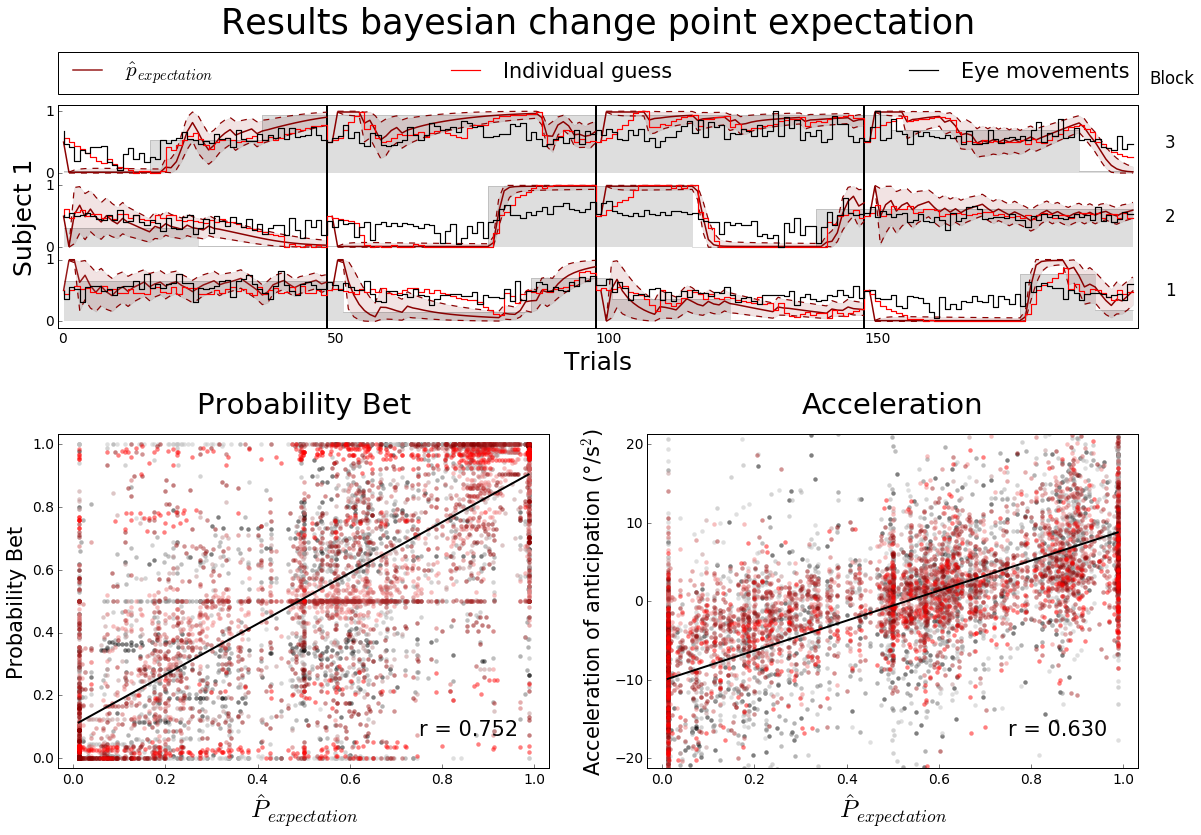
\includegraphics[width=1\linewidth]{results_bayesianchangepoint_e}
\end{center}
\caption{\emph{Analyzing inter-individual differences}
% \textbf{(A)}
% \textbf{(B)}
% \textbf{(C)}
}
\label{fig:results_inter}
\end{figure}
%-------------------------------------------------------------%
We have fitted the sequence generated by each participant and
for each session, that is for eye movements and the rating scale.
The scatter plot of the best fit values are shown in~\seeFig{results_inter}.
It first shows that there is some variability in the best fit value of $\tau$
in both sessions.
If the average is close to the (hidden) value used to generate the sequence
(with $\tau = XX \ms \pm XX \ms$ for the first session and
 $\tau = XX \ms \pm XX \ms$ for the second),
 we observe a variability which is characteristic of the spectrum of individual choices.
More importantly, there is a slight but consistant
correlation between the values for each participant for one session
as compared to the second session.
% TODO - Granger / transfer entropy
Also we have found that using measures of causality,
the results for eye movements slightly lagged before
that of the rating scale,
suggesting that there could be an advance
It can serve as a biomarker...

%: %%%%%%%%%%%%%%%%%%%%%%%%%%%%%%%%%%%%%%%%%%%%%%%%%%%%%%%%%%%%%%%

\section{Discussion}


%The oculomotor system has to constantly update its knowledge about the environment. An ordeal is then to adapt to changes with the shortest delays. Early studies have proposed that stimuli provides information to modulate reaction times within sequences~\citep{Hyman1953, Tune1964, Schvaneveldt}. This theoretical approach is coherent with the notion of local transition probabilities that quantifies at which extent an observation deviates from the preceding ones~\citep{Meyniel2016}. The way expectations act on cognitive processes has been investigated by a wide range of domains such as predictive coding~\citep{Wolpert2000, Wacongne2012}, active inference~\citep{Friston2010}, motor control~\citep{Sutton1998, Behrens2007} and reinforcement learning~\citep{Nassar2012}. Non-stationary observations can also explain why both local and global effects emerge and why local effects persist in the long run even within purely random sequences~\citep{Cho2002, Yu2009}. This constant update of a general belief on the world can be a consequence of the constant attempt to learn the non-stationary structure of the environment that can change at unpredictable times~\citep{Yu2009}. Many studies have actually already pointed the brain's ability to apprehend non-stationary states in environments~\citep{Ossmy2013, Meyniel2015}. As explained by~\citet{Meyniel2016}, the belief upon an environment can be divided in two different ways:
%
%\begin{enumerate}[label=\Alph*)]
%\item Update the~\textit{a priori} likelihood of a sudden change, also known as the volatility and taken into account by the model~\citep{Behrens2007}
%\item A leaky integrator factor imbedded in the model~\citep{Anderson2006, Yu2009, Ossmy2013, Wang2002}
%\end{enumerate}
%

%: theory / computationnally-driven experiments
% it's a main novelty
genrative models for changing environments allows to know the ground truth compared to natural stimulation (see Rust eand Movshon)%
Let's remember our hierarchical generative model.

At any given trial, we wish to construct an algorithm which

We will introduce a fundamental component of Bayesian models : a latent variable

this new variable will be used to test different hypothesis which will be evaluated to predict future states. it is called latent because it aims at representing a variable that is latent (or hidden) to the observer

in our case, we will assume that the bayesian model knows about the structure of the generative model and we will set it to the current run-length $r$, that is, at any given trial, the hypothesis that the past r observations belong to the same block. of course a wrong choice of a latent variables (let's say the temperture in the experimental room) may give unexpected results, even is the bayesian model is "optimal" - an essential point to understand in bayesian inference

extension to multi-nomioal( daniele + fred danion)



% Still, only Bayesian models recover an explicit probabilistic representation of change in likelihood. Recent experimental studies suggest, indeed, that the brain is able of estimating a hierarchical model of the environment and that humans can explicitly report sudden changes in sequences~\citep{Meyniel2015, Gallistel2014}. Ultimately, we passed over one of leaky integrator models' main default, having a too fixed and rigid memory parameter. In our work the memory parameter is constantly inferred by the BCP algorithm over the observation of the number of trials where this inference stayed reliable and then globally represented probabilistic representation of changes in likelihood and actualization of~\textit{a priori} knowledge.


perspectives:
- RL : use hindsight example of localization for saccades: get the changepoints then improve estimate of reward allows to optimize the association between the set of measures and their utility (compared to Q-learning where it is a fixed length)
- interindividual differences : markers for the berhaviour traces - traces of the network implementation
- the brain is weakly Bayesian (it does not care about equations but more about sugar)


%: %%%%%%%%%%%%%%%%%%%%%%%%%%%%%%%%%%%%%%%%%%%%%%%%%%%%%%%%%%%%%%%

\section{Conclusions}


\begin{itemize}\setlength{\itemsep}{0ex}
\item There is a strong correlation between the real probability and the value of the bet,

\item there is a stong correlation between the strength of anticipation and the probability of the process,

\item we have developed a Bayesian model of an agent estimating the probability of changing points. This allows to dynamically infer the direction probability and directly compare model and human behaviour.

% to summarize, we have shown that
% - there is a correlation in the anticiapatory response of eye movements
% in a volatile environment that is captured if we know the true probability
% - that a fixed length models captures some of this correlation, but that
% - our online bayesian changep[oint model better captures this correlation
% and that this may hint at the neural mechanisms used to anticipate
% in a dynamic environment
%
% the brain is not strongly a bayesian machine, but weakly

\end{itemize}
%: %%%%%%%%%%%%%%%%%%%%%%%%%%%%%%%%%%%%%%%%%%%%%%%%%%%%%%%%%%%%%%%
\section{Material and Method}
%%%%%%%%%%%%%%%%%%%%%%%%%%%%%%%%
%%%%%%%%%%%%%%%%%%%%%%%%%%%%%%%%
\subsection{Psychophysics}
%%%%%%%%%%%%%%%%%%%%%%%%%%%%%%%%



% TODO replace this with the actual protocol using psychopy

%cf. https://github.com/chloepasturel/AnticipatorySPEM/issues/19
\textbf{Stimuli were generated using PsychoPy 1.85.4 on a Mac running OS 10.6.8 (A VERIFIER) and displayed on a 20" Viewsonic p227f monitor (A VERIFIER) with resolution $1280\times 1024$ at 100~\si{\Hz} (60 ?). Psychophysics routines were written using PsychoPy 1.85.4 controlled the stimulus display. Observers sat 57~\si{\cm} from the screen in a dark room. Twelve observers (29 years old +/- 5.15) with normal or corrected-to-normal vision took part in these experiments. They gave their informed consent and the experiments received ethical approval from the Aix-Marseille Ethics Committee in accordance with the declaration of Helsinki.}
%Stimuli were presented on a 21 inches CRT monitor with refresh rate of 100 Hz. Stimuli were generated using the Psychophysics Toolbox extension for Matlab (Brainard, 1997; Pelli, 1997) running on a Mac Pro (first generation) computer and displayed at a viewing distance of 57 cm against a gray background. The luminance of the gray background was 42 cd/m2. To minimize measurement errors, the subject’s head movements were restrained using a chin and forehead rest, so that the eyes in primary gaze position were directed towards the center of the screen. Eye movements were measured continuously with an eye tracking system (Eyelink 1000, SR Research Ltd., sampled at 1000 Hz) and data were transferred, stored, and analyzed offline using programs written in Matlab or Ipython notebooks.
%Recorded horizontal and vertical gaze position were low-pass filtered using a Butterworth (acausal) filter of order 2 with a 30 Hz cut-off frequency and then were numerically differentiated to obtain velocity measures. We used an automatic conjoint acceleration and velocity threshold method to detect saccades (Krauzlis & Miles, 1996) and further inspected all individual traces visually to exclude aberrant trials. Saccades were excluded from eye velocity traces (and replaced by NaN values in the numerical arrays) before trial averaging. We evaluated the effects of the experimental manipulations on anticipatory velocity at the individual level, by comparing the mean eye velocity during a critical time window, between –50 and +50ms around target motion onset (as highlighted in Figure 2), using individual one-way ANOVAs (with the probability bias or reinforcement type as 3-levels single factors). We also computed all post-hoc pair-wise comparisons using Tukey’s HSD test. Even though the normality assumption of our data was fairly justified given the sample’s size (always over 60 trials per condition), we also computed non-parametric statistics (Kruskal-Wallis test) for comparison and results were similar. All tests and analyses have been realized using Python 3.5 with the Numpy and Scipy libraries.
3 blocks of 200 trial - with 4 sub-blocks of 50 trials


 * the whole experiment was coded by Chloé using :
 - python for the generative model,
 - the psychopy library for the stimulus display + connection to the eyelink 1000 that we used to record EMs
 - numpy, pandas and pylab for the data analysis

  * all this code is available : for running the experiments, re-analyzing the data and doing all plots are on github

These python scripts are available at \url{https://github.com/chloepasturel/AnticipatorySPEM}.


We asked subjects to perform two tasks on different days :
%\begin{itemize}\setlength{\itemsep}{0ex}
%\item a <<Bet>>
%\item a <<recording>>
%\end{itemize}

In summary, the design of our experimental setting is therefore very similar to the previous experiment but with a more general construct:

- using the same 3-layered generative model, we generated sequences of directions

- and generated 3 blocks of 200 trials

- with an average block length of 40 trials

We anticipated that such an  experiment for which we simply recordedd the eye movements should be more difficult for observers compared to the classical experiments with longer (400 trials), fixed blocks and...

\subsection{The Bet}
In this first part, the subjects must simply answer before each trial at the question \textit{ ``How sure are you that the target will go left or right''}. This was performed by adjusting a cursor on the screen using the mouse (see Figure).

%\textbf{ Un point de fixation blanc de 10px de large est affiché au début d'un essai. Les sujets doivent ajuster le curseur sur une échelle blanche gradué placé en desous. Cette échelle présente 3 graduations : 'gauche' et 'droite' au extrémité et 'incertain' au millieu. Pour validé leurs choix, les sujets doivent cliquer sur la souris. L’échelle et le point de fixation disparaissent et une cible en mouvement à 15°/s (voir pour LB$_Bet$ 20°/s) s’affiche à l’écran. La cible est un cercle blanc mesurant 10px de large et 2px de lineWidth.}


%\textbf{Lors de cette tâche les mouvement oculaire sont enregistré à 100 Hz via Eyelink 100. Le module Python Pylink (SR research) 0.1.0 nous a permis de faire le lien entre Eyelink et nos routines python. Les sujets ont la tête fixe, et on leur demande de ne pas cligner des yeux lorsque le stimuli aparait. Chaque essais commence par la présentation d’un point de fixation blanc de 10px de large au centre de l’écran pendant une durée variable de 400 à 800 ms. Si le signal enregistré n'est pas présent dans une fenêtre de $120\times 120$ px autour du point de fixation ou si il n’est pas stable (clignement, mauvais enregistrement…), la durée de fixation recommence. À la fin de cette durée de fixation il y a un GAP de 300ms, le point de fixation disparait laissant juste un écran gris. Puis une cible en mouvement de 15°/s apparaissait de sorte que 100ms après sont apparition il soit au centre de l’écran, afin d’évité la première saccade. La cible est un cercle blanc mesurant 10px de large et 2px de lineWidth (REDONDANT).}


This is why we added a supplementary experiment for each observer but on a different day for which we asked at every trial to give a subjective, conscious evaluation of the direction of the next trial + a confidence about this inference. Once this information given by the subject, we were showing the actual outcome.

Interestingly, we used exactly the same sequence, allowing to make a direct comparison of the results of both experiments

We called this experiment the bet experiment.


\textbf{Tous les 50 essais le 'score' du sujet sur les 50 derniers essais est affiché au centre de l'écran, le sujet doit appuyer sur la barre espace du clavier pour continuer (doit dire a l'expérimentateur quand il veux continué, on ne pouvais pas brancher une souris et un clavier en même temps). Ce score est égal à $\sum_{x=0}^{50} \frac{Bet_{x} \times dir_x}{50} \times 100$. Où $Bet_x$ est le parie du sujet à chaque début d'essaie comprie entre -1 pour la gauche et 1 pour la droite, $dir_x$ est la direction de la cible pour chaque essai, -1 pour la gauche et 1 pour la droite.}


%\subsection{The Bet}
%Example of results obtained during the bet :
%\begin{center}
%    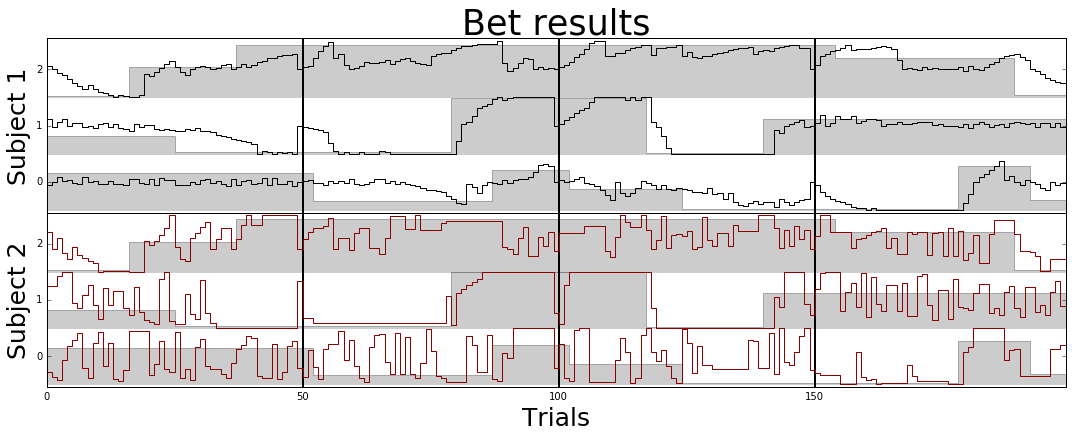
\includegraphics[width=1\linewidth]{results_pari}
%\end{center}
%%Comparison of probabilities bet with respect to the real probability :
%The scatter plot of the value of the bet (probability bet) as a function of the real probability at every given trial shows that there is a good correlation between both values:

%\begin{center}
%    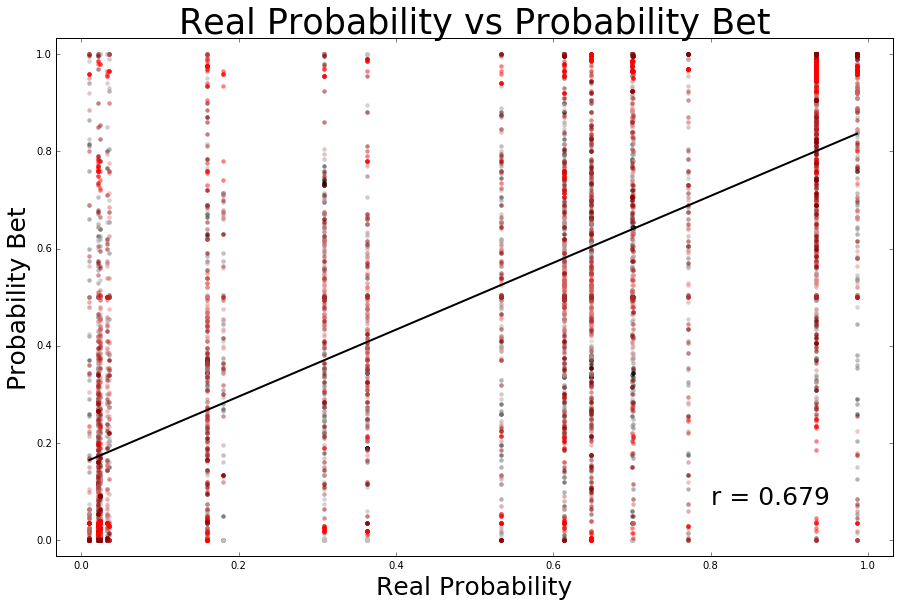
\includegraphics[width=1\linewidth]{p_real--p_bet}
%\end{center}

\subsection{Eye movements recording}

%
%Experiment 1: motion direction-bias task (Baseline)
%	 The visual stimulus used in experiment 1 was a white ring (0.30° outer diameter and 0.23° inner diameter) with a luminance of 102 cd/m2 that moved horizontally on a grey background. Each trial started with a central fixation point displayed for a random duration drawn from a uniform distribution ranging between 300 and 600ms. Then a fixed-duration 300ms gap occurred between the offset of the fixation point and the onset of the moving target, which was presented at the fixation location and immediately started moving horizontally at a constant speed of 7.7 °/s, either to the right or to the left for 1000 ms. Across experimental sessions, the probability P of rightward trials was manipulated in order to create a direction bias and favor the buildup of direction expectancy (See Figure 1A). The experiment included three sessions. The first session had P=0.50, hence about 200 rightward trials out of 400 trials; the second one had P=0.75 (about 300 rightward trials out of 400 trials); the last one P=0.90 out of a total of either 400 (360 rightwards) or 600 trials (540 rightwards) (respectively 9 and 10 participants). The rationale for having a larger number of trials in the P=0.90 session was to collect enough trials for the least frequent direction, namely the left one, but after running the first participants, we realized that the detailed analysis of the least-frequent trials did not provide per se a major advantage for the present study, since the anticipatory behavior was clearly observable with the standard 400 trial-sessions. As we wanted to test a condition without any direction uncertainty, four participants also completed an additional session of 400 rightward trials only (P=1.00). With the exception of the P=1 condition, target motion direction was pseudo-randomized across trials once for each session type, such that all participants were presented with the exact same sequence of randomly alternating directions. Participants were instructed to track the target as accurately as possible.
%
%
Then, we recorded their eye movements as they were tracking the target's motion. Importantly, we used that exact same sequence.

% TODO replace this with the actual protocoml using psychopy
%Stimuli were generated using Matlab 7.10.0 on a Mac running OS 10.6.8 and displayed on a 20" Viewsonic p227f monitor with resolution $1024\times 768$ at 100~\si{\Hz}. Psychophysics routines were written using Matlab and Psychtoolbox 3.0.9 controlled the stimulus display. Observers sat 57~\si{\cm} from the screen in a dark room. Six male observers with normal or corrected-to-normal vision took part in these experiments. They gave their informed consent and the experiments received ethical approval from the Aix-Marseille Ethics Committee in accordance with the declaration of Helsinki.

In parallel, we are developing new automatic routines for the advanced analysis of oculomotor traces. In order to extract the relevant parameters of the oculomotor responses (latency, gain, initial acceleration, catch-up saccades), we developed new tools based on best-fitting procedure of predefined patterns (i.e. the typical smooth pursuit velocity profile).

These python scripts are available at \url{https://github.com/invibe/ANEMO}.


\subsection{Eye movements analysis}

In order to extract the relevant parameters of the oculomotor responses, we developed new tools based on a best-fitting procedure of predefined patterns and in particular the typical smooth pursuit velocity profile that was recorded for the aSPEM (Top row). This was applied to each trial individually, and we show below some prototypical example of respectively a neutral, anticipatory positive and anticipatory negative aSPEMs examples (respectively second to bottom rows).
%%%%%%%%%%%%%%%%%%%%%%%%%%%%%%%%
%: %%%%%%%%%%%%%%%%%%%%%%%%%%%%%%%%%%%%%%%%%%%%%%%%%%%%%%%%%%%%%%%
\section{Appendices}
%%%%%%%%%%%%%%%%%%%%%%%%%%%%%%%%
%%%%%%%%%%%%%%%%%%%%%%%%%%%%%%%%
\subsection{Appendix 1: Analysis of eye movements}
\label{app:em}
%%%%%%%%%%%%%%%%%%%%%%%%%%%%%%%%




I show here a typical velocity traces for one subject / 2 trials

- x-axis is time in milliseconds aligned on target onset,
and we show respectively from left to right the fixation in gray,
the GAP in pink (300ms) and the run in light gray.

- y-axis is the velocity as computed as the gradient of position.
Remark that the eyelink provides with the periods of saccades or
 blinks that we removed from the signal. it is quite noisy and
 to complement existing signal processing methods,
 Chloe implemented a robust

- fitting method which allows to extract some key components of
the velocity traces: maximum speed, latency, temporal inertia ($\tau$)
 and most interestingly acceleration before motion onset.
 We cross-validated that this method was givinfg similar results
  to other classical methods but in a more robust fashion/

While being sensible to recording errors, this allows us to extract the
 anticipatory component of SPEMs and..


%%%%%%%%%%%%%%%%%%%%%%%%%%%%%%%%
\subsection{Appendix 2: Mathematical proof}
\label{app:bcp}
%on $\[O, 1\]$ or is Jeffrey's prior  $\Jj = BB(\frac 1 2 , \frac 1 2 )$~\seeApp{bcp}(TODO: put in appendix). There is always a switch at t=zero.

%%%%%%%%%%%%%%%%%%%%%%%%%%%%%%%%
%%%%%%%%%%%%%%%%%%%%%%%%%%%%%%%%
\subsection{Appendix 3: Supplementary psychophysical results}
\label{app:results_psycho}
%\seeApp{results_psycho}
%%%%%%%%%%%%%%%%%%%%%%%%%%%%%%%%

%%%%%%%%%%%%%%%%%%%%%%%%%%%%%%%%
{\tiny
\printbibliography
}
%%%%%%%%%%%%%%%%%%%%%%%%%%%%%%%%
%%%%%%%%%%%%%%%%%%%%%%%%%%%%%%%%
\end{document}%
